\documentclass[a4paper, twoside, 12pt]{report}

\usepackage[english]{babel}
\usepackage[utf8x]{inputenc}
\usepackage[T1]{fontenc}
\usepackage{listings}
\usepackage{hyperref}
\hypersetup{colorlinks=false}
\usepackage{lscape}
\usepackage{subfigure}
\usepackage{amsmath}
\usepackage{graphicx}
\usepackage[colorinlistoftodos]{todonotes}
% Added later - for table in appendix
\usepackage[normalem]{ulem}
\useunder{\uline}{\ul}{}
\usepackage{longtable}

% Bibliography Harvard Style
% Use this and change the style to agsm / apalike / lsalike
%\usepackage{natbib}

% Break-line for URLs
\def\UrlBreaks{\do\/\do-}
\usepackage{breakurl}

% Table spacing
\usepackage{verbatimbox}

% Another table package
\usepackage{tabulary}
\usepackage{adjustbox}

% Image positioning
\usepackage[section]{placeins}

% Code printing
\usepackage{color}
\usepackage{listings}
\usepackage{caption}

\newcounter{nalg}[chapter] % defines algorithm counter for chapter-level
\renewcommand{\thenalg}{\thechapter .\arabic{nalg}} %defines appearance of the algorithm counter
\DeclareCaptionLabelFormat{algocaption}{Algorithm \thenalg} % defines a new caption label as Algorithm x.y

\lstnewenvironment{algorithm}[1][] %defines the algorithm listing environment
{   
    \refstepcounter{nalg} %increments algorithm number
    \captionsetup{labelformat=algocaption,labelsep=colon} %defines the caption setup for: it ises label format as the declared caption label above and makes label and caption text to be separated by a ':'
    \lstset{ %this is the stype
        mathescape=true,
        frame=tB,
        numbers=left, 
        numberstyle=\tiny,
        basicstyle=\scriptsize, 
        keywordstyle=\color{black}\bfseries\em,
        keywords={,input, output, return, datatype, function, in, if, else, foreach, while, begin, end, write, store, get, do, calculate, test, on, } %add the keywords you want, or load a language as Rubens explains in his comment above.
        numbers=left,
        xleftmargin=.04\textwidth,
        #1 % this is to add specific settings to an usage of this environment (for instnce, the caption and referable label)
    }
}
{}
% /Code printing

%% Sets page size and margins
\usepackage[a4paper,top=3cm,bottom=2cm,left=4cm,right=4cm,marginparwidth=1.75cm]{geometry}

\title{Predicting music popularity}
\author{Rares Dinu}
% Update supervisor and other title stuff in title/title.tex

\begin{document}
\begin{titlepage}

\newcommand{\HRule}{\rule{\linewidth}{0.5mm}} % Defines a new command for the horizontal lines, change thickness here

%----------------------------------------------------------------------------------------
%	LOGO SECTION
%----------------------------------------------------------------------------------------
 
%----------------------------------------------------------------------------------------

\center % Center everything on the page

%----------------------------------------------------------------------------------------
%	HEADING SECTIONS
%----------------------------------------------------------------------------------------
\quad\\
%\textsc{\LARGE MSc Thesis}\\[1.5cm] % Name of your university/college
\textsc{\huge University of Manchester}\\[0.2cm] % Major heading such as course name
\textsc{\Large School of Computer Science}\\[0.5cm] % Minor heading such as course title
\textsc{\large 3rd Year Project Report}\\[0.5cm]

%----------------------------------------------------------------------------------------
%	TITLE SECTION
%----------------------------------------------------------------------------------------
\makeatletter
\HRule \\[0.5cm]
{ \huge \bfseries Predicting Music Popularity}\\[0.4cm] % Title of your document
\HRule \\[1.5cm]

\includegraphics[width=5.5cm]{title/logo.png}\\[1cm] % Include a department/university logo - this will require the graphicx package
%----------------------------------------------------------------------------------------
%	AUTHOR SECTION
%----------------------------------------------------------------------------------------

\begin{minipage}{0.4\textwidth}
\begin{flushleft} \large
\emph{Author:}\\
Rares Dinu % Your name
\end{flushleft}
\end{minipage}
~
\begin{minipage}{0.4\textwidth}
\begin{flushright} \large
\emph{Supervisor:} \\
Prof. Gavin Brown 
% Uncomment the following lines if there's a co-supervisor
%\\[1.2em] % Supervisor's Name
%\emph{Co-Supervisor:} \\
%Dr. Adam Smith % second marker's name
\end{flushright}
\end{minipage}\\[3cm]
\makeatother


%----------------------------------------------------------------------------------------
%	DATE SECTION
%----------------------------------------------------------------------------------------

{\large A dissertation submitted for the degree of}\\[0.2cm]
{\large \emph{BSc Computer Science with Industrial Experience}}\\[1cm]
{\large \today}\\[2cm] % Date, change the \today to a set date if you want to be precise

\vfill % Fill the rest of the page with whitespace

\end{titlepage}

\begin{abstract}
Ever since the music industry has started to be profitable, artists and record labels alike have been looking for the secret recipe of a hit song. The aim of this paper is to find out whether popular songs can be predicted by looking at features of the audio itself or derived from it provided by the Spotify API using machine learning classification algorithms. An in-depth analysis of the algorithms available, the model selection process, the data used and the feature selection and parameter optimisation processes is provided. The results were promising, showing it might indeed be possible to make such a prediction, the best model for the task being the SVM. Some features that were more prominent in the prediction were also identified and those seemed to be energy, loudness, tempo and duration. To showcase the results, a web application was implemented where a user can search for a song on Spotify and see the results of the prediction of different models.
\end{abstract}

\renewcommand{\abstractname}{Acknowledgements}
\begin{abstract}
Throughout the course of this project I have received a great deal of support and assistance. I would first like to express my gratitude to my supervisor, Prof. Gavin Brown, whose guidance and expertise was invaluable and helped me remain focused and eager to learn for the whole duration of the project. I would also like to thank my family and my girlfriend for their unconditional love and constant encouragement.
\end{abstract}

\tableofcontents
\listoffigures
\listoftables

%\chapter{Introduction}
This is one of the most important components of the dissertation. It should begin with a clear statement of what the project is about so that the nature and scope of the project can be understood by a lay reader. It should summarise everything you set out to achieve, provide a clear summary of the project's background and relevance to other work and give pointers to the remaining sections of the dissertation which contain the bulk of the technical material.

Further information can be found here: \url{https://goo.gl/k2huN9}.

\section{\LaTeX{} code examples and formatting tips}
Hello, here's a citation. References are stored in a Bibtex file. Google Scholar and IEEExplore allow you to download citations of papers in Bibtex format from their search engine. Some people use JabRef (\url{http://www.jabref.org}) to manage their database of references.

This is an inline equation $\Gamma(t)=K_i e^{\sin^2(\omega_t)}$. The first paragraph appears without indent but the following ones will have an indentation.

This is an actual named equation:
\begin{equation}
v(x)=\frac{1}{2}\sin(2 \omega t + \phi) e^{-j s t}
\label{eq:cacona}
\end{equation}
\noindent where $\omega$ is the angular speed. Notice that symbols liks $\omega$ should be written in italics whereas measurement units such as V for Volts appear as normal text. This paragraph didn't have an indentation because the first sentence was linked to the definition of equation (\ref{eq:cacona}). A code snippet for an example program is shown in Listing~\ref{lst:code1}.

\begin{lstlisting}[caption=Source code for {\it hello.m},label=lst:code1,breaklines=true,basewidth=4pt,prebreak=**,postbreak=**,frame=single]
for i:=maxint to 0 do
begin
{ do nothing }
end;
Write('Case insensitive ');
Write('Pascal keywords.');
\end{lstlisting}

The characteristic parameters of the system are summarised in Table~\ref{tab:tab1}. A figure is shown Fig~\ref{fig:felix}, we don't necessarily know if this figure will appear below, above or elsewhere; therefore, the text should never refer to the figure with sentences such as {\it "As shown here:"}.

\begin{figure}[htbp]
\centering

\includegraphics[width=0.3\linewidth]{introduction/fig/Felix_the_cat.pdf}
\caption{Felix the Cat}
\label{fig:felix}
\end{figure}

\begin{table}[htbp]
	\centering
	\begin{tabular}{lll}
		Parameter & Value & Units\\
		\hline
		$P$ & 1 & kW \\
		$Q$ & 0 & kVAr\\
	    \hline
	\end{tabular}
	\caption{Characteristic parameters of the system}
	\label{tab:tab1}
\end{table}

\begin{samepage}
Sometimes, the symbols in an equation are defined as follows\footnote{Some authors like to define their symbols this way.}:
\begin{equation}
	V(t)=A \sin(\omega t+\theta_0)
\end{equation}
\begin{tabular}{lll}
	where & $V$ & is a voltage waveform,\\
	& $A$ & is the amplitude of the voltage,\\
	& $\omega$ & is the angular frequency,\\
	& $t$ & is the time.
\end{tabular}
\end{samepage}

\subsection{A brief comparison between a proper plot and a horrible plot}

Figure \ref{fig:fig2} contains two plots of the same waveform. Subfigure \ref{fig:fig2sub1} shows a badly formatted figure, Subfigure \ref{fig:fig2sub2} shows a much better formatted figure. The problems with Subfigure \ref{fig:fig2sub1}, listed by order or relevance, are the following:

\begin{enumerate}
    \item The font size is too small to be read properly.
    \item The axes aren't labeled properly: the horizontal axis is not labeled and the units of the vertical axis are unknown. Further, symbols must be written in italics whereas numbers and units must be written as normal text.
    \item The choice of limits for the axes is not good, the figure has wide useless empty spaces. The most relevant part of the waveform is the transient that happens between times $t=$0 and $t=$0.05 s, which is less than 10\% of the timespan shown in the figure.
    \item The figure has been scaled without keeping the original aspect ratio and fonts look narrower than they would if the figure had been scaled properly.
    \item The plot doesn't have grid lines. This makes it hard to read the exact value (ie time, voltage) of points in the trace.
    \item The width of the trace is too thin and may not be visible if printed in low resolution.
    \item The choice of units of the vertical axis aren't the best. For example, in this case the plot would be easier to read if voltage had been expressed in kV instead of V.
    \item The figure was exported as a bitmap (e.g. png, jpg, bmp) instead of being exported in vector format (e.g. eps, svg, pdf) and visual artifacts appear when the figure is scaled up or down in order to fit in the document.
\end{enumerate}

\begin{figure}[htbp]
	\centering
	\subfigure[A horrible one.]{
		\label{fig:fig2sub1}
        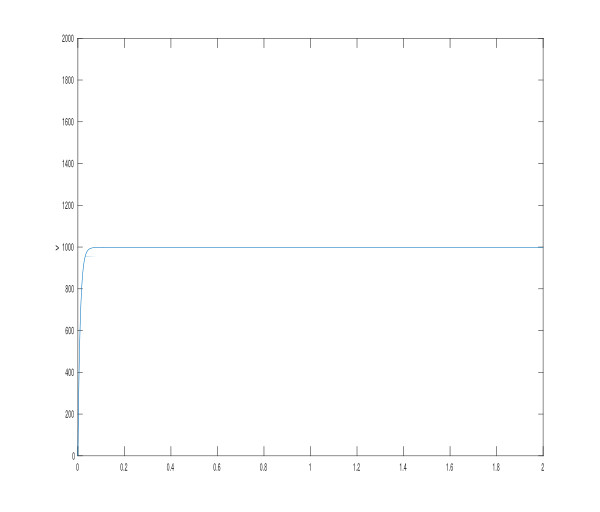
\includegraphics[width=0.5\linewidth]{introduction/fig/figure1.jpg}}
	\subfigure[A proper one.]{
		\label{fig:fig2sub2}
		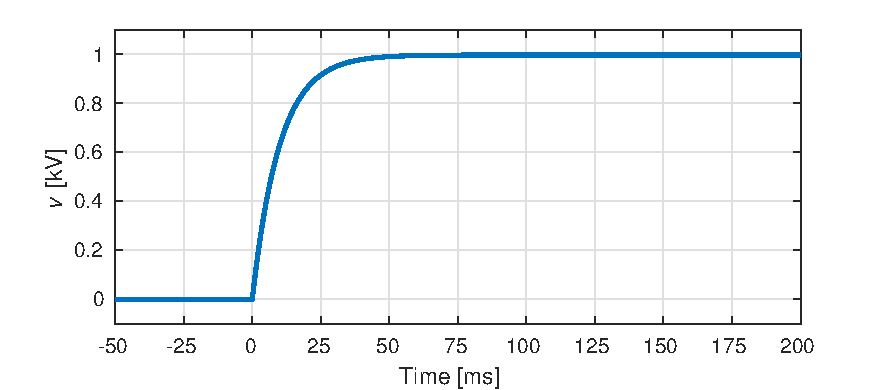
\includegraphics[width=0.6\linewidth]{introduction/fig/figure2.pdf}}
	\caption{A figure with two subfigures.}
	\label{fig:fig2}
\end{figure}

\begin{landscape}
	\begin{figure}[htbp]
\centering

\includegraphics[width=0.4\linewidth]{introduction/fig/Felix_the_cat.pdf}
\caption{Here's a large drawing of Felix the Cat that wouldn't fit in a portrait page}
\label{fig:felix2}
\end{figure}
\end{landscape}

\section{Objectives}
\section{Challenges}
\section{Contributions}
\chapter{Introduction}

This chapter looks at the motivation for this project while also providing a clear generic description of the project and a summary of the aims and the technical achievements.

\section{Motivation}
Music is all around us. Even if we try to, we literally can't get away from it. It's on TV, in shops, in cars and even on the street and with the advances of technology it's only going to become louder and more ubiquitous. People need a soundtrack to their lives. However, there are still a lot of artists who try to make a living by playing music and dream of becoming stars but in their pursuit of fame they struggle to find that sound that could make them famous. But what if they had a tool to help them? People often say that all the songs on the radio sound the same or that music nowadays is very repetitive. As if the people who produce the popular music have found a 'secret recipe' that they just follow blindly, change a few lyrics and melodies and out comes a brand new hit. Could this be true? Could we, using modern technology, determine what aspects all hit songs have in common, and so engineer the ultimate key to musical success? Well, this gave me the initial idea for this project and it was the starting point for my research.

Being passionate about music and knowing that a lot of popular songs tend to use the same chords at their core, just with added elements on top I thought there might actually be some truth to this. But how to prove it? I knew I wanted to use machine learning since I wanted to learn more about it and knew from my experience in university that it could be applied in such a problem. I also knew I wanted to use Spotify since it is a very popular music streaming platform that had a freely accessible API.

Using this technology we can use predictors on the Spotify data to try to find out if there is a link between all hit songs, some prevailing features that can distinguish them from non-hits. If we could do that, then an artist would be able to try the effect of the predictors on their own music and fine tune the song until it has what it takes to be popular. Similarly, a music label looking to sign artists can look at the prediction of an artist's songs and use that insight to inform their decision. With the music industry being incredibly profitable and still continuously growing especially with the rise of paid streaming services such as Spotify and Apple Music \cite{USMusicI78:online}, such predictions would be invaluable to artists, music labels, and even to the media who could use it to pick songs to broadcast that they know their audience will like. It might not be as easy as it sounds and we might not want a society where all the songs released are hits but it is a captivating thought worth exploring.

\section{Summary of project aims}
\begin{itemize}
    \item Find an answer to the question "Is it possible to predict whether a song will be a hit just based on the audio?" by using machine learning and data from Spotify
    \item Find the best classifier, features and parameters for this prediction task
    \item Implement some kind of tool where an artist or music label could see the potential of a piece of music
\end{itemize}

\section{Summary of technical achievements}
\begin{itemize}
    \item Successfully used data from the Spotify API and classification algorithms from the sci-kit learn library to predict popular songs
    \item The model parameters and features were optimised to improve the performance of the predictors
    \item The resulting accuracy of predictions was better than some previous work in this area and concluded that it is indeed possible to predict hit songs with a good degree of certainty
    \item A web application was implemented to showcase the results where a user can see the real time prediction of different classifiers on any song they search for on Spotify
\end{itemize}




\chapter{Background}
In this chapter, a more thorough introduction to the research topic of this project is presented while also discussing related work in the area and introducing the Machine Learning concepts and techniques used.
\section{Hit Song Science}
Perhaps unsurprisingly, this research topic is quite a popular subject that has also gained some attention from the media. This is probably because a few companies have released products that they claimed were able to predict hit songs with high accuracy. This, as you can imagine, would be an invaluable tool for music producers and artists alike since they would be able to use it to their advantage and ultimately make a profit. However, it is unclear if those hit prediction tools actually worked and the implementation details were mostly kept secret.

This field of investigation has been referred to as Hit Song Science, a term coined by Mike McCready, founder of a music analysis company, and it aims to predict the success of songs before they are released on the market. However, as it turns out, there might be more to predicting the popularity of songs than just the features of the audio itself. Psychological aspects also come into play and a wide range of factors such as exposure, music marketing, media broadcasts, social influence play a role in whether we like a song or not. That is because what we listen to might be influenced by what our friends listen to, by what is played on radio/television or by what is being more heavily marketed. It is also usually the case that songs of popular artists will also be popular since they already have the exposure, while a new, unknown artist might struggle to get their songs on the radio since the popular songs get all the airtime (the rich get richer and poor get poorer). 

This makes the whole prediction problem even more complex than it was already. However, in Hit Song Science and, consequently, in this project, the goal is to look at the relation between features of the audio and the popularity of that song while disregarding these aforementioned complex and confusing psychological aspects. This problem then becomes similar to the prediction of stocks or the weather. Another way to look at this, as Pachet, puts it is "...as an idealistic attempt to determine the 'objective causes' of individual music preference, independently of the effects of social influence"  \cite{li_music_2011}.

\section{Related work}
\label{sec:relatedwork}
Research in this area has gone back and forth over time with some studies claiming that this kind of prediction might be possible and others saying that it is not. One of the earliest attempts is the work of Dhanaraj and Logan \cite{dhanaraj2005automatic}. They used general acoustic features (based on Mel-frequency cepstral coefficients) and features extracted from lyrics. To classify hits they used Support Vector Machines (SVMs) and boosting classifiers and for the data they used a database of 1700 songs. After the study, they concluded that there might indeed be something that distinguishes hits from non-hits and that audio based features and lyrically based features perform well on their own, but result in poorer performance when combined. 

Later, a larger scale and more complete study by Pachet and Roy \cite{pachet2008hit} contradicted their results. They used a database of 32000 songs with features from the MPEG-7 audio standard, a specific acoustic set generated with proprietary algorithms and a set of high-level metadata manually produced by humans. The classifier used was also SVM with an RBF kernel so the main differences were the features used and the size of the dataset. This study concluded that the popularity of songs cannot be learned from features of music titles, in this way contradicting the claims of Hit Song Science. This experiment could have put end to the debate on the topic due to its scale and level of completeness but as it turns out it might have had the opposite effect, fuelling even more experiments since it did not disprove the hypothesis completely \cite{li_music_2011}.

\begin{figure}[h]
\centering
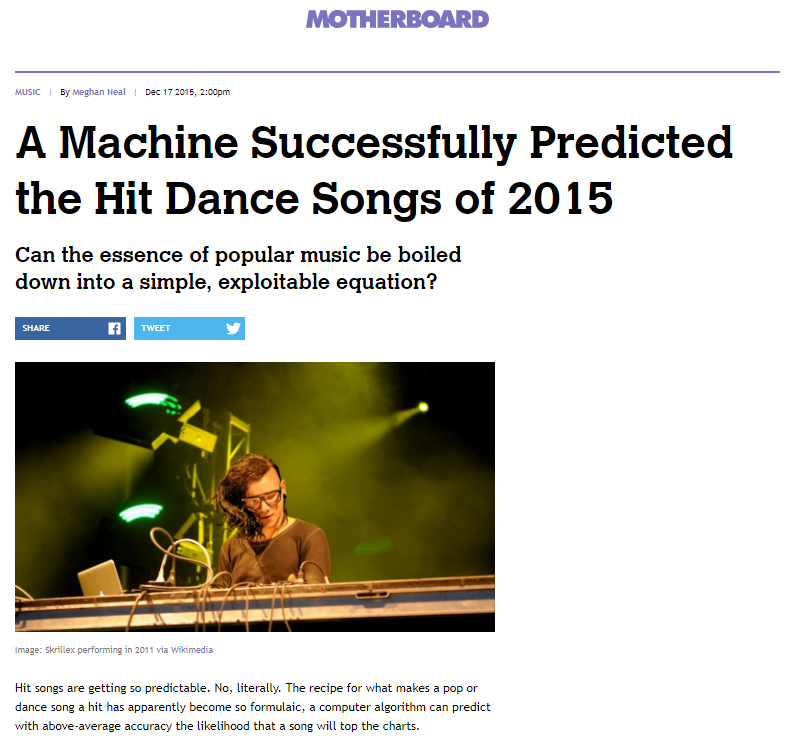
\includegraphics[width=0.50\linewidth]{background/fig/art2.PNG}
\caption{Online artice about the study of Herremans et al. \cite{herremans2014dance} \cite{MachineArticle:online}}
\label{fig:hitarticle}
\end{figure}

Trying to distinguish the top 5 from top 30-40 hits, Ni et al. \cite{ni2011hit} showed an experiment with more optimistic results due to the slightly different approach, the more novel audio features used (extracted from the EchoNest API, a music intelligence platform) and the classifier (a time-shifting perceptron). They claimed that hit song science might be a science once again. The research, however, does not include a lot of the perhaps important details of the implementation. Another study was conducted by Herremans et al. \cite{herremans2014dance} that looked at a similar approach, trying to predict if a song is a top 10 dance hit. Therefore, it only focused on a particular genre. The features were also obtained from The Echo Nest. They used models such as C4.5 trees, RIPPER rule set, logistic regression and SVMs, the best performing being the logistic regression model. This experiment again showed promising results concluding that predicting the popularity of dance songs is possible and is due to only using recent songs (so there is no need to account for the change in music taste over time), focusing on one genre and the features used.

More recently, Pham et al. \cite{pham2016predicting} used a subset of 2700 tracks from The Million Song Dataset \cite{bertin2011million} with features from this data set plus some from The Echo Nest. They compared different classifiers concluding that the SVM with an RBF kernel was the best performing one. Their aim was to also find the features that were more prominent in the prediction. Again, their study showed good results and the features that were more powerful predictors seem to have been the metadata ones rather than the acoustic ones since they seemed to reflect the trait of a song more accurately. An even more recent research by Reiman and Ornell \cite{reiman2018predicting} took an approach similar to the one in this project. They looked at predicting hit songs using four different classifiers with a data set of 600 tracks from the Billboard Hot 100 charts and features from the Spotify API. Their results were not as good as some of the previously presented experiments but were still slightly better than a random predictor.

\begin{figure}[h]
\centering
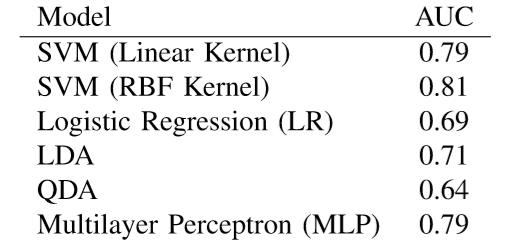
\includegraphics[width=0.7\linewidth]{background/fig/pic1.PNG}
\caption{Classifier AUC score results from the study of Pham et al. \cite{pham2016predicting}}
\label{fig:pham1}
\end{figure}

The results of these experiments seem promising overall making pursuing a different approach at this task worthwhile. While each research seems to have taken a slightly distinct path there were still certain common points. A few papers looked at models such as SVMs, logistic regression, naive bayes, multilayer perceptron, k-nearest neighbors and used features from The Echo Nest. This was a good starting point for my own study.

\section{Classification algorithms}
It seems clear now that some sort of prediction needs to be performed. To do that, this project uses machine learning which is used for the finding of patterns in data in an automated manner \cite{shalev2014understanding}. Nowadays,  we probably encounter machine learning every day when we search the internet, when shop online, even our phones might use it for unlocking using face recognition. It is truly all around us. 

But how do machines learn? Well, in a way similar to how animals or humans do, by using past experience to determine what to do in a new situation. In a very simple example of machine learning, that of filtering spam emails, the machine learning algorithm will be provided with a lot of examples of spam and non-spam messages. It will find patterns in these messages, such as the frequent occurrence of bad words in spam perhaps and when a new email arrives it will be able to tell if it is spam or not by using its 'past experience'. There are two main types of ways in which a machine can learn: supervised and unsupervised. 

Supervised learning applies in situations like the ones described above with the spam filter. Given a sample of messages that are labelled as spam and some labelled as not spam, when a new message arrives it can be labelled according to its similarity to a spam/non-spam message. In Figure \ref{fig:supunsup} a line (usually called a decision boundary) is drawn to separate the two classes. When a new point is plotted, it will be labelled according to which side of the decision boundary it is on.

On the other hand, in an unsupervised task the messages used for training are not labelled and so the algorithm needs to find patterns that separate the messages in a way, by clustering the data set into smaller subsets of similar messages, for example, like in Figure \ref{fig:supunsup} \cite{shalev2014understanding}. 

\begin{figure}[h]
\centering
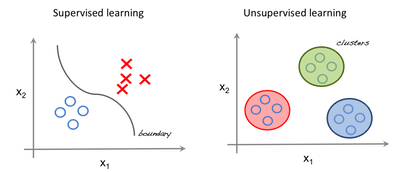
\includegraphics[width=0.9\linewidth]{background/fig/graph.png}
\caption{Supervised and unsupervised learning visualised \cite{SupervisedUnsupervised:online}}
\label{fig:supunsup}
\end{figure}

For the task in this project supervised learning will be used since we will provide the machine learning models with examples of songs that are labelled as popular or not popular. The model should then learn a certain pattern that differentiates popular songs from the less popular ones that it will then be able to apply to a previously unseen song and label it accordingly. 

As a starting point for choosing which classification algorithms to use, the related literature was reviewed. A few research papers used Support Vector Machines, Logistic Regression, Gaussian Naive Bayes, Multi-layer Perceptron and even K-Nearest Neighbours. Those were implemented to be able to compare results with previous work but other models were also tested such as Random Forests and AdaBoost. Below a succinct description of these models is provided.

Logistic regression is a machine learning technique that came from the field of statistics. It is at its core a mathematical modelling approach used to describe the relationship between a set of independent variables and a dependent variable. It is a very popular model because its output is a value between 0 and 1, value which describes a probability since it uses a sigmoid function (Equation \ref{eq:logreg}) to map predicted values to probabilities. The output represents the likelihood of the example belonging to class 1. For example, if predicting whether an individual has a disease or not, the probability will indicate how likely it is that the individual has that disease \cite{kleinbaum2002logistic}.

\begin{equation}
f(z)=\frac{1}{1+e^{-z}}
\label{eq:logreg}
\end{equation}

\addvbuffer[12pt 8pt]{
\begin{tabular}{lll}
	where & $e$ & is Euler's number,\\
	& $z$ & is the input to the function(the algorithm's prediction).\\

\end{tabular}
}


K-Nearest Neighbours is one of the simplest algorithms in machine learning, yet it is quite effective. To predict the class of a new given point, it looks at its k nearest neighbours (where k can range from 1 to the total number of points minus one and is usually chosen depending on the data). It then uses a majority vote to decide on the class of the new point \cite{16Neares99:online}.

Support Vector Machines are a "machine learning tool used for learning linear predictors in high dimensional feature spaces" \cite{shalev2014understanding}. It tries to find an optimal hyperplane to separate the given classes. The hyperplane is optimal when the distance between the hyperplane and the training examples is maximum. For example, in two dimensions the hyperplane would be a line that separates the points as seen in \autoref{fig:svm} and in three dimensions it would be a plane \cite{Introduc22:online}.

\begin{figure}[h]
\centering
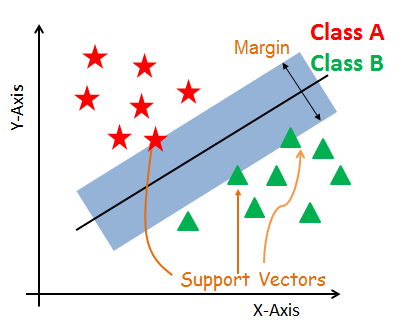
\includegraphics[width=0.6\linewidth]{background/fig/svm.PNG}
\caption{SVM application on 2D data \cite{SVMGraph:online}}
\label{fig:svm}
\end{figure}

The multi-layer perceptron (MLP) is a type of artificial neural network. As the name suggests, it is built upon the simpler perceptron which is a linear classifier that models a biological neuron. A multi-layer perceptron is composed of more than one perceptron which makes it able to solve more than just linear prediction tasks. An input layer receives the signal (the input data) and an output layer makes a decision based on the input. Between those two layers there can be any number of hidden layers that handle the bulk of the computation \cite{ABeginne87:online}.

The Naive Bayes classifiers are a family of simple probabilistic classifiers. Despite their simplicity they are very popular and have proven very effective. They use Bayes' theorem but with the added naive assumption that all the features are independent of each other, in other words, they assume conditional independence. This is considered a "naive" approach because it very rarely applies to the real world \cite{zhang2004optimality}. Gaussian Naive Bayes comes as an extension of the naive Bayes that adds the capability of handling continuous variables by making the assumption that the features are generated using a single Gaussian distribution \cite{john1995estimating} \cite{reiman2018predicting}.

The Random Forest or Random Decision Forest is an ensemble learning method, which means it uses multiple classifiers, in this case decision trees, to classify the data and then takes a majority vote of all those classifiers to decide on the class of an example. In this way, it mitigates the tendency of decision trees to overfit the data, improving the generalisation accuracy \cite{ho1995random}.

The AdaBoost classifer \cite{freund1997decision}, short for Adaptive Boosting, is a machine learning ensemble meta-algorithm that essentially tries to obtain a strong classifier from a set of weak ones. It trains a classifier on the data set and then creates new instances of that classifier that are trained on the same data set but the weights of incorrectly classified instances are adjusted (hence the adaptive title) \cite{sklearnadaboost:online}.

These algorithms were then implemented using the \textit{sci-kit learn} library \cite{pedregosa2011scikit} in Python. It is a module for machine learning that features various classification, regression and clustering algorithms including the ones mentioned above but also many more. Furthermore, it is designed to work with other numerical libraries in Python such as NumPy and SciPy. The code is run using Jupyter Notebooks \cite{kluyver2016jupyter}, a document format in which code from different languages can be executed. It is based around the IPython kernel which can run the Python code in Jupyter. It works in a browser and it provides a way of integrating code, explanations (in the form of text) and results (in the form of plots or graphics) in a single document which makes for easy reading, executing and understanding.

\section{Feature selection}

Feature selection is the process of removing the features that are not helpful to the predictor from the data. Often times this can improve the performance of the model since features that are not relevant can have a negative impact on the predictions. We are interested in only keeping the features that have the highest contribution to the desired output \cite{FeatureSel:online} \cite{guyon2003introduction}. There are three main types of methods used for feature selection: wrapper methods (use the model to score different feature subsets), filter methods (select feature subsets in the preprocessing phase, without using the model) and embedded methods (specific models can perform feature selection as part of training). 

Since the data only has 13 features the best feature subset can be found searching exhaustively by calculating a score for every possible feature combination and picking the best one. This is a wrapper method. There are therefore \(2^{13} - 1\) possible feature subsets and for each of them an AUC score is calculated using cross validation. Then the process is repeated for every model since the features chosen depend on the model used. The algorithm then looks like Algorithm \ref{alg3}.

\begin{figure}[h]
\centering
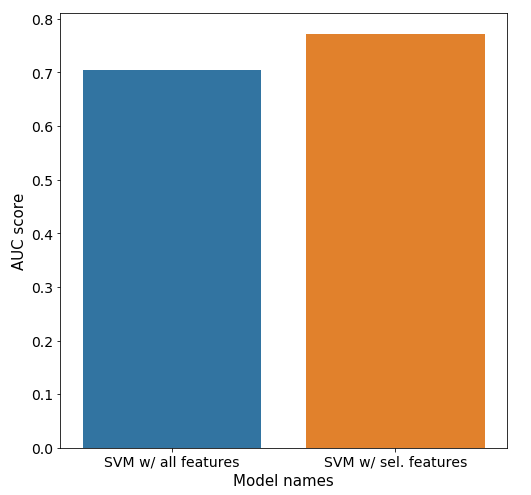
\includegraphics[width=0.8\linewidth]{background/fig/fs1.PNG}
\caption{AUC score for SVM before and after feature selection}
\label{fig:fs1}
\end{figure}

As an example, the performance increase for SVM can be seen in Figure \ref{fig:fs1} with the score plotted for the classification being performed on data with all the 13 features and on data with 7 selected features (energy, tempo, speechiness, instrumentalness, time signature, duration, loudness). It is about a 7\% increase which may not be much but the reduction of features leads to a much simpler model, the number of features being almost halved.

\begin{algorithm}[caption={"Feature selection algorithm"}, label={alg3}]
begin
    foreach model in the model list
      foreach possible feature subset
        do cross validation
          calculate AUC score for each iteration
        end
        calculate average AUC score for all iterations
        store feature set and score in a list
      end
      pick subset with best score for model
    end
end
    
\end{algorithm}

\section{Imbalanced classes}
\label{sec:imbalance}
Early on when trying to evaluate the models the results seemed unusually high. That was because I was only looking at the prediction accuracy of the models which is the percentage of correct predictions. That was a problem since almost 90\% of the data set is of class 0 and only 10\% of class 1 so it is highly imbalanced (this can be observed in Figure \ref{fig:imbalance}). This meant that if the model predicted everything as class 0 it would have a 90\% accuracy even though it failed to identify any of the hits which is what we are actually interested in. To mitigate this problem a few different approaches were tried: using over-sampling, adjusting class weights in models and looking at different scoring metrics (discussed in Section \ref{sec:evalation}).

\begin{figure}[h]
\centering
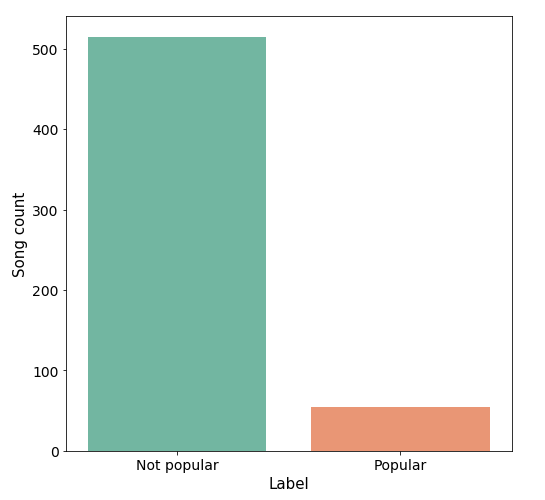
\includegraphics[width=0.7\linewidth]{background/fig/imbalance.PNG}
\caption{Plot of number of examples for each class in the data set}
\label{fig:imbalance}
\end{figure}

Over-sampling is a technique used to create more examples of the minority class to make the data set balanced. A common way to do so was to just duplicate the examples of the minority class, but this can easily lead to overfitting. A better approach is SMOTE (Synthetic Minority Over-sampling Technique) \cite{chawla2002smote}, a technique used to create new "synthetic" samples by using an algorithm similar to k-nearest neighbours that creates a new example and randomly sets its feature values based on those of the neighbours. 

Another technique that can be used to mitigate this problem involves adjusting the model to penalise a misclassification of a sample of class 1 more than one for class 0. This can be done by adjusting the weights of the classes and some models in sci-kit learn support a parameter that sets the weights automatically according to the balance of samples in the data set.

Both of these options were used and compared to ensure the best solution was chosen. The scores were similar with slightly higher results when adjusting the weights but since that was not available for every model, over-sampling also had to be used. 


\chapter{Methodology}

This chapter takes an in-depth look at the methodology used in this project. It covers the way the data is obtained, the features used, and a discussion on what to consider a hit song. It also take a closer look at the data to see what can be learned just by analysing it on its own and how it needs to be prepared for the machine learning algorithms to work better. Finally, the evaluation measures are presented and the training and testing protocols are explained along with the optimisation of the hyperparameters of the models.

\section{Description of data sources}
Spotify \cite{kreitz2010spotify} is one of the largest music streaming services available today with about 200 million monthly active users. In 2014, Spotify bought Echo Nest \cite{SpotifyEchoAquisition:online} which was a music intelligence and data platform and along with it, it got a database of 30 million songs \cite{TheEchoN16:online} containing data aggregated from web crawling, data mining, and digital signal processing techniques. As seen in Section \ref{sec:relatedwork}, The Echo Nest API was a common source for data in related research in this area. It now powers Spotify's music recommendation and playlist curation features. It is worth mentioning that with it being such a popular streaming service nowadays, artists or record labels use it as one of their main distribution platforms and so upload the music to the service to release it to the world. Spotify also provides an API to query that database and get information about any song. 

The data used in this project was all made available by this freely available Spotify Web API \cite{WebAPI:online}. The API allows access to information about songs in their database such as song title, artist name, etc. but also contains a different endpoint to get information derived by their music intelligence algorithms. 

For each song that is added on their platform they store the usual metadata such as artist name, song title, release date, album cover, etc. but also calculate a range of audio features using signal processing and some proprietary algorithms. There are 13 such features and those are: duration, key, mode, time signature, acousticness, danceability, energy, instrumentalness, liveness, loudness, speechiness, valence and tempo. Some of these are direct features of the audio(such as duration) but others (such as dancebility) are calculated by Spotify and provide more abstract measures. A more in depth explanation of each of those features can be found in Table \ref{tab:feature}.
Since these features are calculated for every song in their database they can be used to compare the songs with each other and as input for the machine learning models.

To query the API a Python script was created with the \textit{spotipy} library \cite{Spotipy:online} (a lightweight Python library for the Spotify API) that really simplified the interaction. The database of songs is truly huge but the songs vary a lot in genre, year of release, popularity, language and we need a subset that is representative of listening trends nowadays. For this project it was important that the songs represent the current popularity trend so a playlist was manually created using the Spotify Desktop Application. This playlists aggregated the top 50 songs on Spotify from various countries (US, UK, Brazil, Romania, France, Germany, etc.) to account for different tastes in music in different regions and had 600 songs. For each song the metadata and the audio features described above are retrieved and stored in a csv file. The algorithm is presented in pseudocode in Algorithm \ref{alg1}.
\begin{algorithm}[caption={"Getting the data"}, label={alg1}]
begin
    foreach song in the playlist
        get song metadata from API
        get song audio features from API
        store the information as a new row
    end
    write data to csv
end
    
\end{algorithm}

\section{Establishing the ground truth}
\label{ground_truth}
One of the very important questions that had to be answered early on was what exactly is a hit song or what it is considered to be in this research. Looking at related work, there have been a few different ways of approaching at this. Some studies used charts like the ones from Official Charts Company \cite{herremans2014dance} or Billboard Top 100 \cite{reiman2018predicting} considering a song a hit if it appeared on these charts. Others used a "song hotttnesss" metric from The Echo Nest API that ranged from 0 to 100 and set a threshold to consider everything above 75 to be popular \cite{pham2016predicting}. This project uses a metric provided by the Spotify API called \textit{popularity}, similar to the "song hotttnesss". This is a score between 0 and 100 calculated by Spotify using the number of plays a song gets and how recent those plays are. So, a very popular song should have a score of 100 and an unknown song should have a score close to 0 but even if a song has a lot of plays but those plays are not recent it will score low. This is useful since it also provides an insight into what the current trend is.

I chose to consider every song with a popularity of 90 or more as popular (class 1) and everything below that threshold as not popular (class 0). This threshold was chosen since we want to distinguish the truly popular songs, the top 10 percent, from the rest since that represents a more useful prediction. A lower threshold also resulted, based on experimentation, in poorer results. Based on that threshold value, binary labels are added to the songs. After cleaning the data of duplicates and entries with invalid values the data set has 570 songs out of which 55 songs are labelled as popular and 515 are not popular.

\section{Data insights}
Before applying machine learning, it is useful to plot features against each other to see if any information can be gained from the data itself.

\begin{figure}[h]
    \centering
    \begin{minipage}{0.45\textwidth}
        \centering
        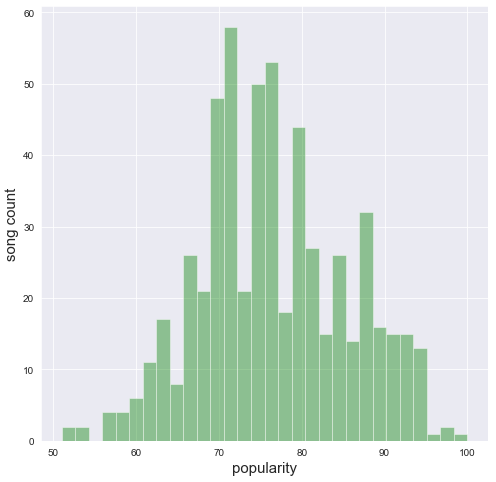
\includegraphics[width=0.9\textwidth]{methodology/fig/histogram.PNG} % first figure itself
        \caption{Popularity histogram}
        \label{fig:histo}
    \end{minipage}\hfill
    \begin{minipage}{0.45\textwidth}
        \centering
        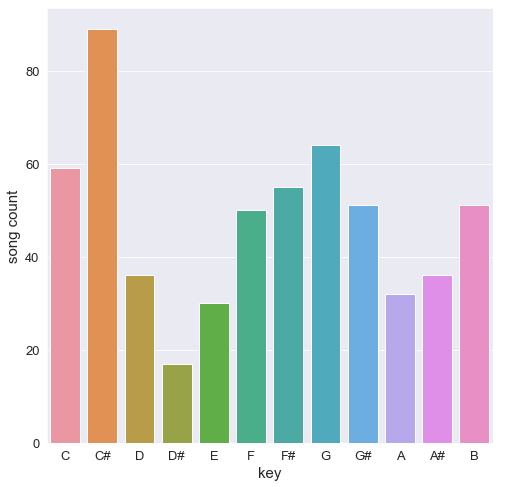
\includegraphics[width=0.9\textwidth]{methodology/fig/keycount.PNG} % second figure itself
        \caption{Key spread in data}
        \label{fig:keycount}
    \end{minipage}
    \begin{minipage}{0.45\textwidth}
        \centering
        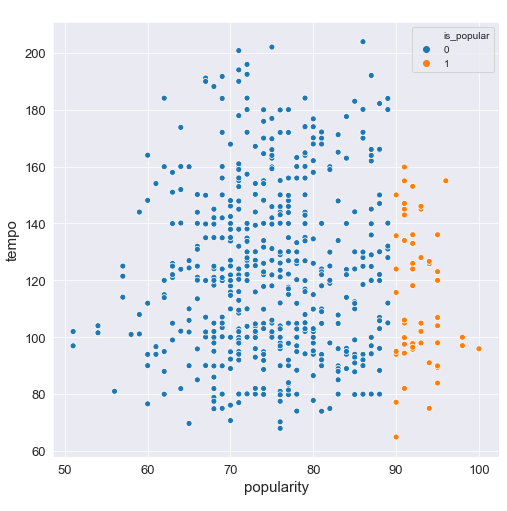
\includegraphics[width=0.9\textwidth]{methodology/fig/temppop2.PNG} % third figure itself
        \caption{Tempo and popularity}
        \label{fig:temppop}
    \end{minipage}\hfill
    \begin{minipage}{0.45\textwidth}
        \centering
        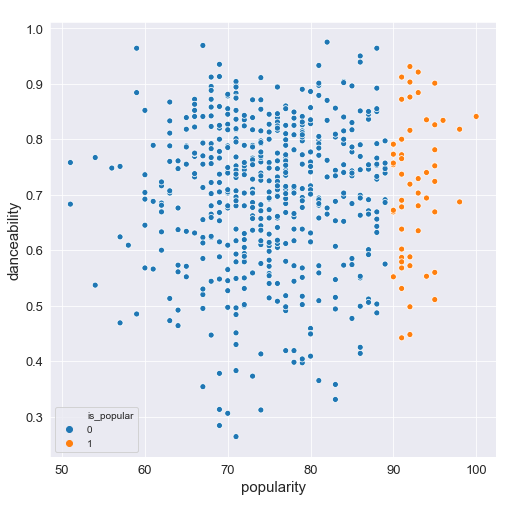
\includegraphics[width=0.9\textwidth]{methodology/fig/dancepop.PNG} % fourth figure itself
        \caption{Danceability and popularity}
        \label{fig:dancepop}
    \end{minipage}
\end{figure}

In Figure \ref{fig:histo} it can be observed that most of the songs in this data set lie in the 70 to 80 popularity range and in Figure \ref{fig:keycount} it can be seen that the keys C\# and G seem to be more common, while D\# is the least common. While there are no very distinct clusters, using Figure \ref{fig:temppop} and Figure \ref{fig:dancepop} some basic assumptions can be made such as if a song has a very high tempo or very low danceability it is likely not popular.

\section{Data pre-processing}
Before the data can be used in the machine learning algorithms it is important that it is scaled so that all the features are brought to the same level of magnitude. This is essential since some algorithms calculate the distance between points using Euclidean distance and each feature should contribute approximately proportionally to the final distance. Scaling is applied for all the features and each scaled feature value is calculated like in Equation \ref{eq:scaling}.

\begin{equation}
z\ =\ ( x\ -\ u) \ /\ s
\label{eq:scaling}
\end{equation}
\addvbuffer[12pt 8pt]{
\begin{tabular}{lll}
	where & $z$ & is the scaled feature value,\\
	& $x$ & is the feature value before scaling,\\
	& $u$ & is the mean of the feature,\\
	& $s$ & is the standard deviation of the feature.
\end{tabular}
}

In Figure \ref{fig:beforesca} and Figure \ref{fig:aftersca} the difference between non-scaled and scaled data can be observed. The data still has the same shape but the values on the y-axis are much smaller after scaling in Figure \ref{fig:aftersca}. The standard deviation and mean can also be calculated without transforming the data so that the transformation can be applied at a later point. This is useful since we might want to scale the test set separately but still apply the same transformation applied to the training data.

\begin{figure}[h]
    \centering
    \begin{minipage}{0.45\textwidth}
        \centering
        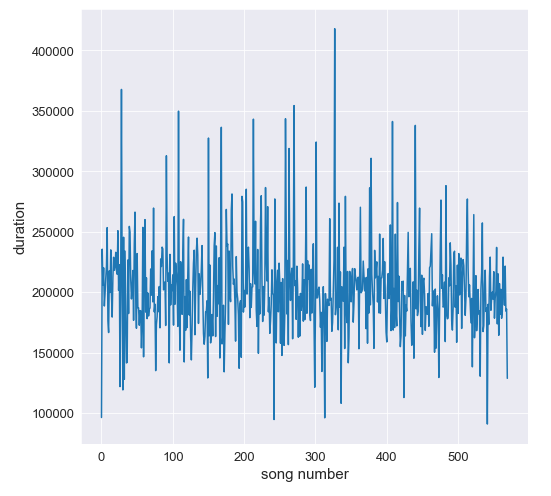
\includegraphics[width=0.9\textwidth]{methodology/fig/beforescaling.PNG} % first figure itself
        \caption{Duration before scaling}
        \label{fig:beforesca}
    \end{minipage}\hfill
    \begin{minipage}{0.45\textwidth}
        \centering
        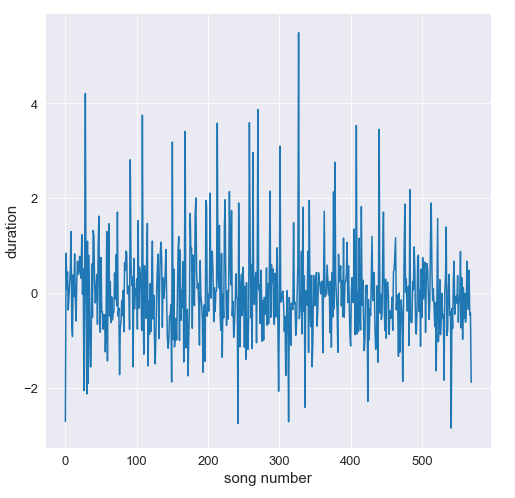
\includegraphics[width=0.86\textwidth]{methodology/fig/afterscaling.PNG} % second figure itself
        \caption{Duration after scaling}
        \label{fig:aftersca}
    \end{minipage}
\end{figure}

With the data scaled, it is now ready to be used by classification algorithms.

\section{Evaluation measures}
\label{sec:evalation}
Since accuracy can be misleading (as discussed in \autoref{sec:imbalance}), other metrics were also used to evaluate the models. Some metrics derived from the confusion matrix such as precision, recall, specificity and F1-score (a weighted average of precision and recall \cite{sklearnm18:online}) were inspected but mainly the Area Under the Receiver Operating Characteristic Curve (AUROC) \cite{bradley1997use} \cite{fawcett2006introduction} was used. The ROC curve represents the True Positive Rate plotted against the False Positive Rate for every possible classification threshold (also called the decision threshold - the value above which an example is considered to be of class 1 - 0.5 by default). The true positive rate is also called recall and it is a measure of how often the prediction is positive when the actual label is 1. The false positive rate is equal to 1 - specificity and it is a measure of how often the prediction is positive when the actual label is 0. The curve can also be seen as a plot of the hit rate versus the false alarm rate. A good classifier would have a curve that spans the upper left corner while a random predictor would have a curve that looks more like the identity line. An example of an ROC curve can be seen in Figure \ref{fig:rocsvm}. AUROC or simply AUC is a good way of measuring the performance of that classifier based on the ROC curve and it tells us how capable the model is of distinguishing between the two classes \cite{ROCAUC:online}. This is a better way of evaluating models because while accuracy only represents the score for one threshold this looks at all the possible thresholds. A good model will have an AUC score close to 1 meaning it is able to separate the two classes while a random predictor would have a score closer to 0.5.

\section{Training and testing protocols}

Since the classifiers have been picked, the next steps in the model selection process are the training and testing of the models. They need to be trained so they can learn and be tested so we can make sure that the pattern they have learned is indeed useful and does not only apply to the input data. That phenomenon is known as overfitting and it means that the model learns a rule that applies too tightly to the training set and will not work well in the real world. To reduce the chances of that happening, a technique known as cross validation is used. Cross validation splits the data set into equally sized chunks called folds. One fold will be left out for testing and the rest are used for training. This process is repeated until every fold has been used for both training and testing as shown in Figure \ref{fig:cv} for five folds. The cross validation strategy used in this project, shuffles the training examples and tries to ensure the same balance of classes in the folds (ten in this case) as in the whole data set \cite{SratifiedCv:online}. 

\begin{figure}[h]
\centering
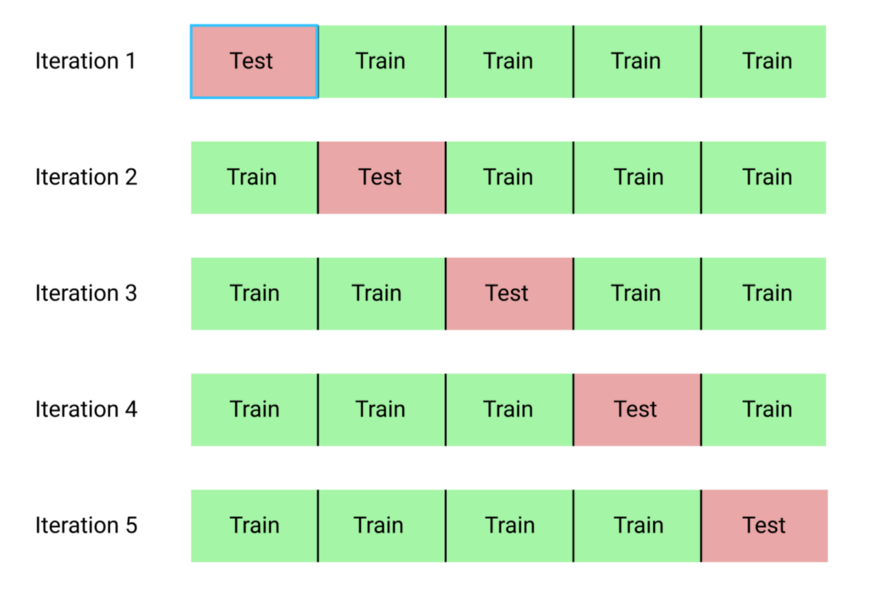
\includegraphics[width=0.7\linewidth]{methodology/fig/cv.png}
\caption{Cross validation process \cite{CrossVal24:online}}
\label{fig:cv}
\end{figure}

\begin{algorithm}[caption={"Model selection algorithm"}, label={alg2}]
begin
    foreach model in the model list
      do cross validation on model selection data set
        calculate score for each iteration
      end
      calculate average CV score for all iterations
      test model on world set
      calculate generalisation score
    end
    choose best model
end
    
\end{algorithm}



Before the cross validation process, the data set is first split into two sets. A bigger one for the cross validation (the model selection set in Figure \ref{fig:modelsel}) and a smaller one (the world set) that will be used for testing. To know how well the models will generalise, how well they will perform in the real world, the smaller subset of data will be kept unseen by the cross validation process to further test the models. That will give an additional indication of whether the models have overfitted the data or not. The whole process is visually described in Figure \ref{fig:modelsel} and algorithmically in pseudo-code in Algorithm \ref{alg2}.

\begin{figure}[h]
\centering
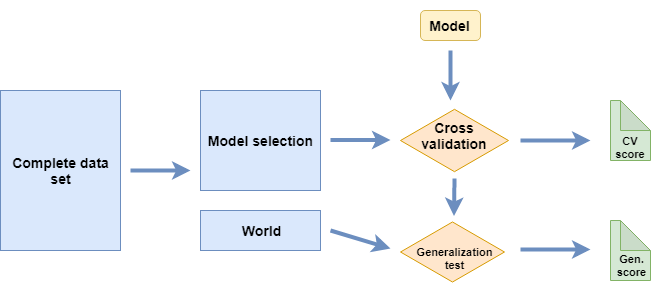
\includegraphics[width=0.9\linewidth]{methodology/fig/process.png}
\caption{Data split for model selection and process diagram \cite{CrossValVimeo:online}}
\label{fig:modelsel}
\end{figure}



\section{Hyperparameter optimisation}

To squeeze every little bit of performance out of the models we can look for the best parameters for the learning algorithms. To do so, Grid Search and cross validation are used. Grid search works similarly to the feature selection algorithm \ref{alg3}. A list of parameters and parameter values like in Figure \ref{fig:hyper} is provided for every model and the algorithm loops through all the possible combinations, calculating scores for each of them. After it is done the best scoring parameter combination is picked.

\begin{figure}[h]
\centering
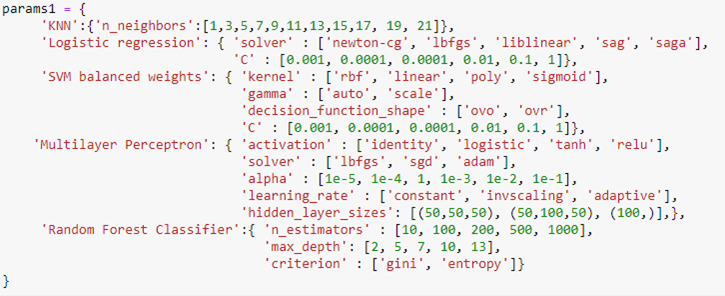
\includegraphics[width=0.9\linewidth]{methodology/fig/hyper.png}
\caption{Example of parameter lists provided for models to be used for Grid Search}
\label{fig:hyper}
\end{figure}

The features selected might influence the parameters chosen and the parameters might influence the features so ideally both of these operations should be done at the same time. This would greatly increase the computation time and might not even be feasible. In this project, a basic manual parameter optimisation was done before the feature selection process and the grid search algorithm was ran to fine tune those parameters on the chosen features after.

Some of the outcomes of this process on this data are, for example, that the best performing kernel for SVMs is the RBF kernel, the best solver for MLP and Logistic Regression is the lbfgs solver and the optimal number of estimators for the Random Forrest is 100.
\chapter{Results and analysis}

In this chapter, the quantitative result data of the model selection process is presented and discussed along with diagrams that show a visual representation of the performance of the models.

\begin{figure}[h]
\centering
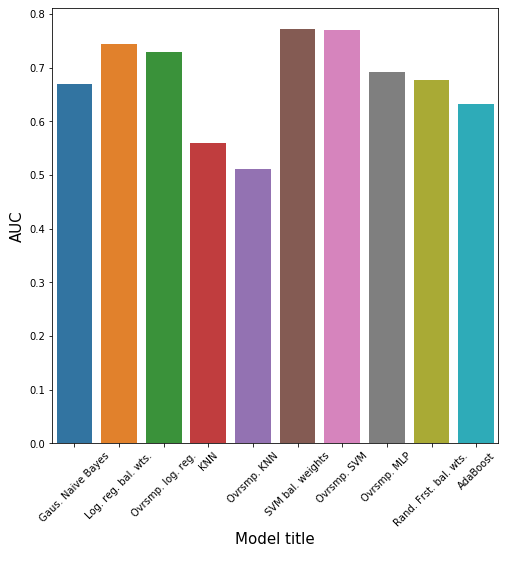
\includegraphics[width=0.9\linewidth]{results/fig/barplot.PNG}
\caption{Model AUC scores}
\label{fig:barplot}
\end{figure}

In Figure \ref{fig:barplot} the AUC scores of all the models averaged over 10-fold stratified cross validation are plotted. SVMs are a clear winner, being followed by Logistic Regression and MLP. The SVM with adjusted weights had an AUC score of 0.77 with a generalisation score of 0.56, Logistic Regression obtained 0.74 and 0.43 and the MLP got 0.69 and 0.57. The ROC curve for SVM is presented in Figure \ref{fig:rocsvm} and AUC scores and ROC curves for individual iterations can also be observed, as well as the standard deviation of the curve. The main curve is averaged over the 10 folds of the cross validation process. Similar ROC curves for Logistic Regression and MLP can be observed in Figure \ref{fig:roclog} and Figure \ref{fig:rocmlp}. 

\begin{figure}[h]
\centering
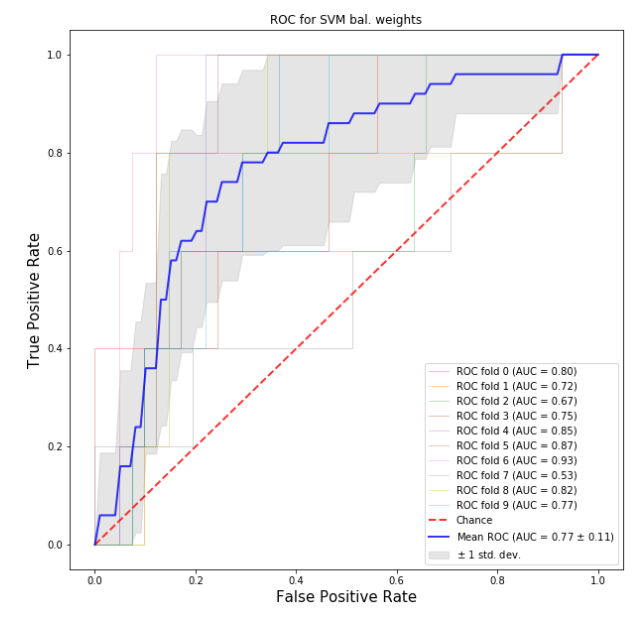
\includegraphics[width=0.7\linewidth]{results/fig/rocsvm.PNG}
\caption{ROC curve for SVM with balanced weights}
\label{fig:rocsvm}
\end{figure}

The Table \ref{tab:modelscores} contains all the metrics calculated for each of the models. When evaluating the performance of the models it is sometimes useful to look at several scores. For example, the MLP with over-sampling has a good AUC score which might indicate at first sight that the model performs well. However, the recall is quite low and that means the model is not good at identifying hits - what we are most interested in. That is also why a score such as the F1 score can be useful since it summarises both recall and precision (the percentage of hits that are correctly classified and the percentage of hit predictions that are correct). A graph with the F1 scores for the models plotted can be found in Figure \ref{fig:f1s}.

\begin{figure}[h]
    \centering
    \begin{minipage}{0.45\textwidth}
        \centering
        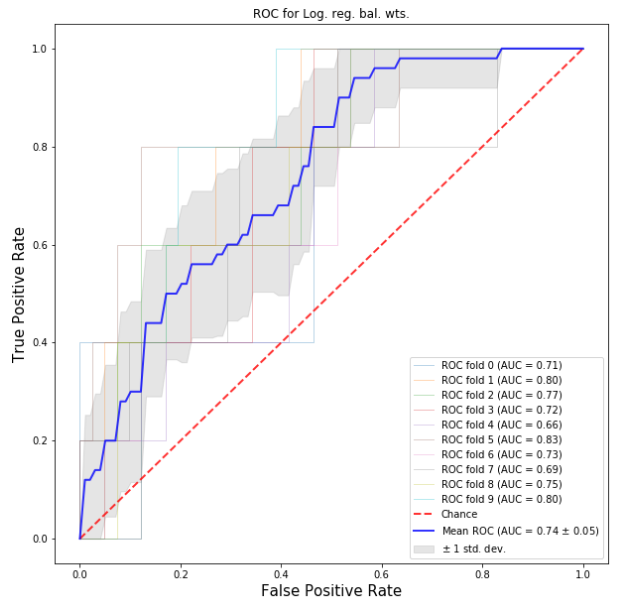
\includegraphics[width=0.9\textwidth]{results/fig/roclog.PNG} % first figure itself
        \caption{ROC curve for Log. Reg. with balanced weighs}
        \label{fig:roclog}
    \end{minipage}\hfill
    \begin{minipage}{0.45\textwidth}
        \centering
        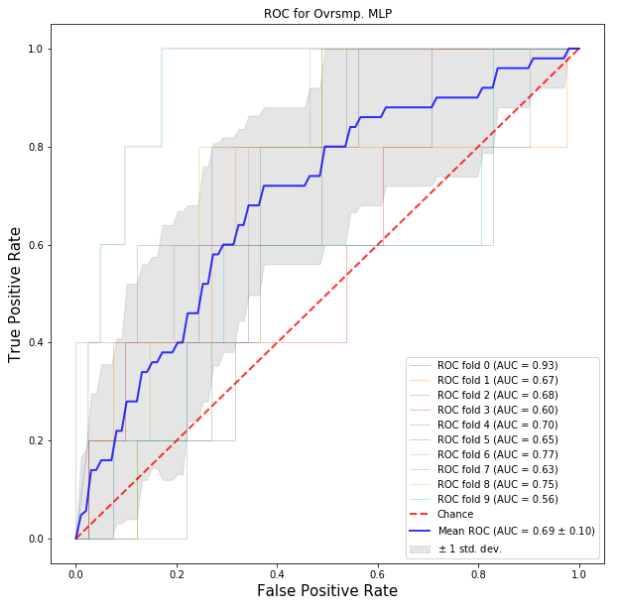
\includegraphics[width=0.9\textwidth]{results/fig/rocmlp.PNG} % second figure itself
        \caption{ROC curve for MLP with oversampling}
        \label{fig:rocmlp}
    \end{minipage}

\end{figure}

The results appear to be in line with some of the previous research where SVMs with an RBF kernel were the best performing model \cite{pham2016predicting}. This means that the data is most likely not linearly separable since the SVM uses something called a kernel trick to map the input into higher dimensional feature spaces. The good performance of some of the other models might be due to the fact that they assumes a linearly separable data space while that might not be the case or due to the particular advantages of the models.

However, due to the variation of experimentation methods in previous research in this area it is hard to accurately compare results. The data sets used are not the same, the features used are different and the way the data is labelled is different. Perhaps this is a further indication to the fact that this is still a field of ongoing research with a plethora of unexplored paths and opportunities. 

I believe the promising results in this project can be due to the smaller data set with recent songs used, the optimisation process and the way the data is labelled (by using the Spotify popularity metric and focusing only on the most popular songs).

\begin{table}[h]
% \begin{adjustbox}{max width=\textwidth}
\resizebox{\textwidth}{!}{%
\begin{tabular}{*{8}{|c}|}
\hline
\textbf{Model title}    & \textbf{Acc.} & \textbf{Spec.} & \textbf{Rec.} & \textbf{Prec.} & \textbf{F1} & \textbf{AUC} & \textbf{Gen. AUC}\\ \hline
Gaussian Naive Bayes    & 0.404             & 0.339                & 0.940                        & 0.149              & 0.257       & 0.670        & 0.421                           \\ \hline
Log. reg. bal. weights. & 0.639             & 0.634                & 0.680                        & 0.191              & 0.296       & 0.745        & 0.433                          \\ \hline
Over-sampling log. reg.  & 0.641             & 0.632                & 0.720                        & 0.194              & 0.304       & 0.730        & 0.454                           \\ \hline
KNN                     & 0.891             & 1.000                & 0.000                        & 0.000              & 0.000       & 0.560        & 0.685                           \\ \hline
Over-sampling KNN        & 0.739             & 0.802                & 0.220                        & 0.130              & 0.159       & 0.511        & 0.478                           \\ \hline
SVM bal. weights        & 0.628             & 0.607                & 0.800                        & 0.203              & 0.320       & {\ul 0.772}  & 0.566                          \\ \hline
Over-sampling SVM        & 0.743             & 0.749                & 0.700                        & 0.270              & {\ul 0.378} & 0.770        & 0.481                          \\ \hline
Over-sampling MLP        & 0.843             & 0.915                & 0.260                        & 0.248              & 0.250       & 0.693        & 0.572                          \\ \hline
Random Forest bal. wts. & 0.733             & 0.768                & 0.440                        & 0.190              & 0.262       & 0.676        & 0.382                           \\ \hline
AdaBoost                & 0.843             & 0.917                & 0.240                        & 0.235              & 0.234       & 0.633        & 0.486                           \\ \hline
\end{tabular}%
}
\caption{Table containing model scores}
\label{tab:modelscores}
\end{table}


\chapter{Web application}

 In this chapter, the web application implemented as a part of this project is presented. Aspects such as the implementation and technologies used are described and the design of the user interface along with the use of the application are discussed. Finally, the evaluation and testing approaches are reported.
 
\section{Architecture and technologies used}
To be able to show the results of the experiment and allow for real time predictions of songs on Spotify a web application was implemented. It allows a user to search for a song on Spotify and see the prediction outcomes of different models. One other feature it has is the model list includes a Multi-layer Perceptron that learns after each prediction so it will improve its performance over time and it should adapt to changing trends.

The popular and unpopular labels, portrayed through the fire and the blue face emoji respectively, express whether the song's features are similar to the features of hit songs or not - if the song has the potential to be popular or not.

Having implemented the models using sci-kit learn with the selected features and optimised parameters, I have used the pickle library \cite{PickleOnline:online} that allows for object serialisation and de-serialisation to save the models to files. I then built a Flask (a Python microframework for web applications) \cite{FlaskOnline:online} back-end and a front end in HTML with Bootstrap and CSS. The user interface is responsive and works on both desktop and mobile. The way the back-end works is: on startup, the back-end loads the models from the files. When a query is sent, it gets the information for a song using the same spotipy library to interface with the Spotify API, applies the machine learning algorithm to that song and returns the resulting prediction to the user where it is displayed using the emoji labels. 

This is the case for all the classifiers except the MLP online one which does some additional operations. After it wrongly predicts a song (the output label is checked against the actual popularity value on Spotify) it will treat that song as a new learning example. In this way, its predictions will improve after each mistake so they adapt to changing trends in music.

\begin{figure}[h]
    \centering
        \centering
        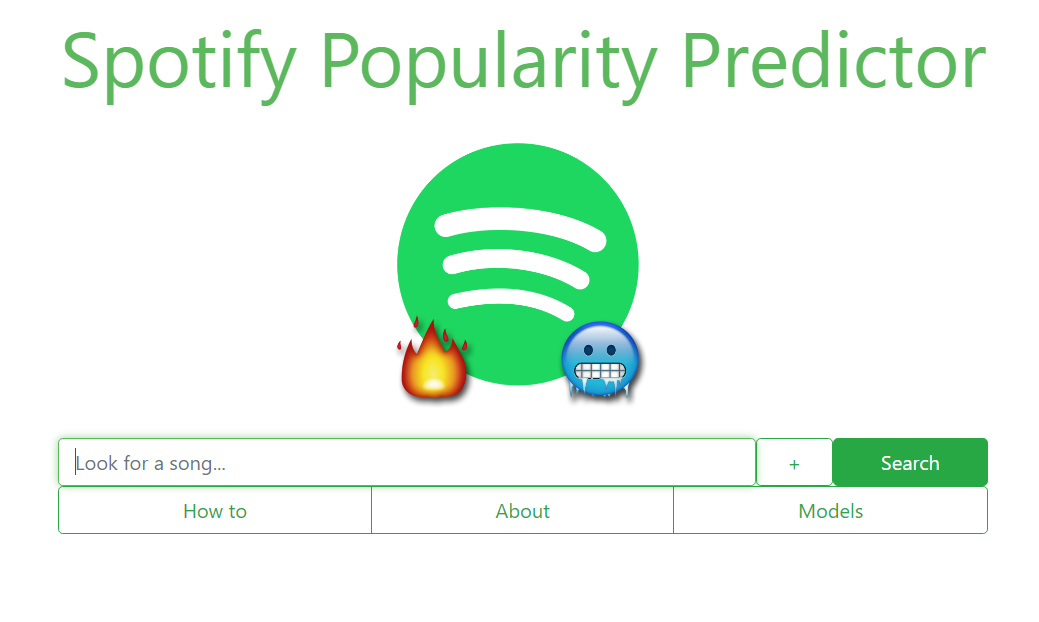
\includegraphics[width=0.8\textwidth]{web_application/fig/ui1.PNG} % first figure itself
        \caption{Landing page}
        \label{fig:ui1}
\end{figure}

% Fix to move content to the next page
% \vspace{40pt}

\begin{figure}[h]
\centering
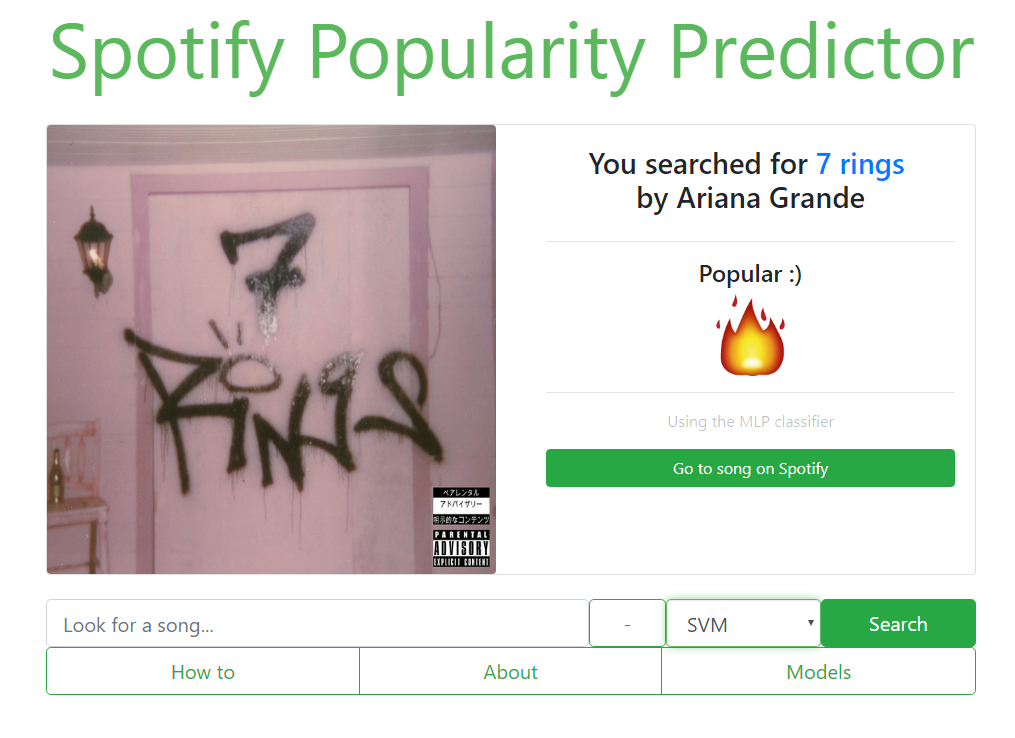
\includegraphics[width=0.8\textwidth]{web_application/fig/ui2.PNG} % second figure itself
\caption{The search performed page for the song "7 rings" by Ariana Grande}
\label{fig:ui2}
\end{figure}

This application is deployed on a cloud platform for Python and is available online \cite{WebApp:online}. It can potentially be used by artists, music labels or the media to see if a song has the characteristics of a hit song, as soon as it is posted on Spotify.

\section{Evaluation}
For the testing of the application different techniques were employed. First, the Audits available in the Google Chrome browser were used to test whether the code respects best practices relating to coding, performance, accessibility and even SEO (Search Engine Optimisation). The report can be seen in Figure \ref{fig:audit1}. The lower score in the Best Practices section relates to the fact that the application does not use the more secure HTTPS which can easily be fixed if it is required. To further ensure code quality, an online HTML validator was used.

The next step was to test the user interface and user experience design. I wanted the user interface to be as minimalistic and consistent as possible, in the same colour theme as the Spotify application and to only allow for simple, obvious interactions. By performing some tests on users such as my supervisor and several friends, some areas of possible improvement became apparent. In an early version of the application, the tabs below the search bar in Figure \ref{fig:ui1} were not implemented so a new user would have no idea what the application does, how to use it and what the results mean. Initially the selection drop-down visible in Figure \ref{fig:ui2} was not hidden so it complicated the interaction of an average user. The design was also changed to include a logo, a bigger title and a horizontal layout in the results page on desktop.

\begin{figure}[h]
\centering
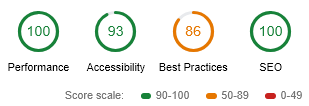
\includegraphics[width=0.6\textwidth]{web_application/fig/audit1.PNG} % second figure itself
\caption{Audit results generated in Google Chrome}
\label{fig:audit1}
\end{figure}

Since the application allows for user input, it is important to test its security even though no sensitive data is stored. Invalid queries are being displayed back to the user but the content is HTML encoded. Also, the Spotify API is used to process those queries so as long as it is secure, the application will also be, so things like database injection techniques will not work because they already have their own safeguards in place. Custom pages for invalid request, page not found, internal server error for the application have also been implemented.

To test the resilience of the application to multiple user interactions, an open source load testing tool \cite{LocustTest:online} was used that allowed the simulation of many simultaneous users. With 100 concurrent users and about 10 requests per second the application performed very well with an average response time of 760 milliseconds across the two main pages and no failures or exceptions. After 200 users some failures started to appear because of the limitations of the web host since the one being used is free but since it is cloud based with an upgrade it could scale for the demand. At 1000 users the failure rate was high but for the same reason as before. Results for the 100 and 200 user cases can be seen in Tables \ref{tab:loadtest1} and \ref{tab:loadtest2}. 


\begin{longtable}{|p{1cm}|p{2cm}|p{1.5cm}|p{1cm}|p{1cm}|p{1cm}|p{1cm}|p{1cm}|}
\hline
\textbf{Met-hod} & \textbf{Name}              & \textbf{\# req.} & \textbf{\# failures} & \textbf{Avg. resp. time} & \textbf{Min resp. time} & \textbf{Max resp. time} & \textbf{Req. /s} \\ \hline
GET             & /                          & 531                  & 0                    & 708                            & 122                        & 7368                       & 5.17                \\ \hline
GET             & /search  & 486                  & 0                    & 817                            & 225                        & 7414                       & 4.73                \\ \hline
                & Total                      & 1017                 & 0                    & 760                            & 122                        & 7414                       & 9.90                \\ \hline
\caption{Statistics of load test for 100 users}
\label{tab:loadtest1}
\end{longtable}

\begin{longtable}{|p{1cm}|p{2cm}|p{1.5cm}|p{1cm}|p{1cm}|p{1cm}|p{1cm}|p{1cm}|}
\hline
\textbf{Met-hod} & \textbf{Name} & \textbf{\# req.} & \textbf{\# failures} & \textbf{Avg. resp. time} & \textbf{Min resp. time} & \textbf{Max resp. time} & \textbf{Req. /s} \\ \hline
GET             & /             & 501                  & 32                   & 6080                     & 120                     & 11739                   & 5.49             \\ \hline
GET             & /search       & 519                  & 23                   & 6519                     & 119                     & 12062                   & 5.69             \\ \hline
                & Total         & 1020                 & 55                   & 6303                     & 119                     & 12062                   & 11.18            \\ \hline
\caption{Statistics of load test for 200 users}
\label{tab:loadtest2}
\end{longtable}

To evaluate the actual prediction results of the web application I started by searching for the top songs on the Spotify charts. Such a query can be seen in Figure \ref{fig:ui2}. That song has been very popular with over 500 million plays on Spotify and the application correctly labels it as popular, therefore the machine learning algorithm correctly identifies the pattern of popular songs in this example and the prediction is what we expect. Also, this particular song is a good example because when the data was sampled, that song had not been yet released. If the application had been used to predict the song upon its release it would have been correct in its prediction. Looking at the most played songs on Spotify from 2013 to present \cite{SpotifyCharts:online}, the application predicts 7 out of the first 10 as popular using the SVM model. 

\begin{figure}[h]
\centering
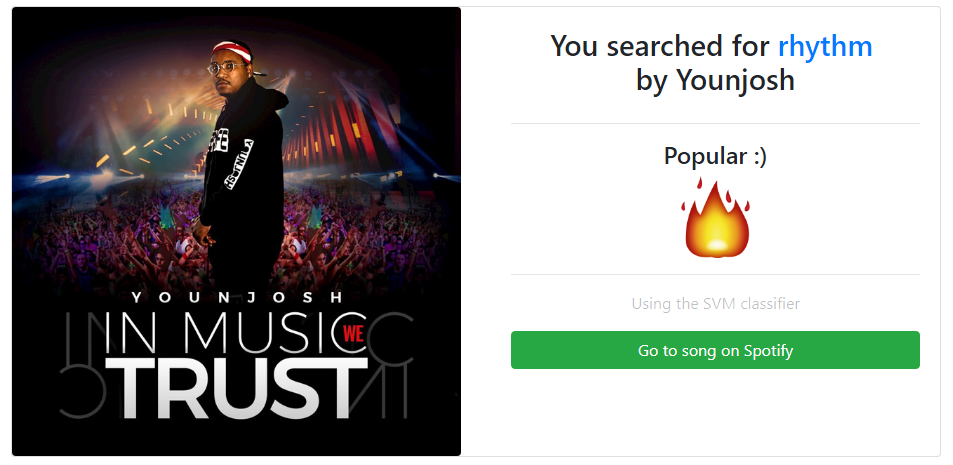
\includegraphics[width=0.7\textwidth]{web_application/fig/ui3.PNG} % second figure itself
\caption{The search performed page for the song "rhythm" by Younjosh}
\label{fig:ui3}
\end{figure}

The next step was to look for some unpopular songs to see if the application can be used to find diamonds in the rough. With less than 1000 plays, the song in Figure \ref{fig:ui3} is clearly not a hit but it was predicted as popular. Hopefully, this song might appear in the charts soon. Interestingly, it uses fragments from an older popular song from the 90's. That result means that the song has features that other hit songs present from an acoustic point of view but maybe other aspects such as the fact that the artist is unknown and lack of promotion come into play so it has not yet become a hit but the algorithm can't consider such aspects. In an ideal world where every piece of music would get the same level of exposure maybe this song could have shined through because of its hit-like features.

The algorithms do sometimes make mistakes so songs get predicted as not popular even though they might be. When this happens I noticed the songs are quite different, maybe unique in some way. The song in Figure \ref{fig:ui4} is a good example, currently being number 1 on the Spotify charts with around 5 million daily plays but it is predicted as not popular. However, the artist is currently very popular and her music is known for being different and unique so again there might be aspects that do not depend on the audio that have contributed to the popularity of this song.

Through testing the application with a lot of different songs, it looks like the performance obtained during the training and testing phase does still apply to the real world. However, to truly see if the application can indeed predict a hit, songs need to be predicted as soon as they are released and their journey followed to see if they do become popular or not which would tell us how reliable those predictions are. To prove the effectiveness of the application this would need to be done for a large number of songs to see how many of the songs predicted as popular upon their release did actually end up popular. This is not that trivial but could be done in the future.



\begin{figure}[h]
\centering
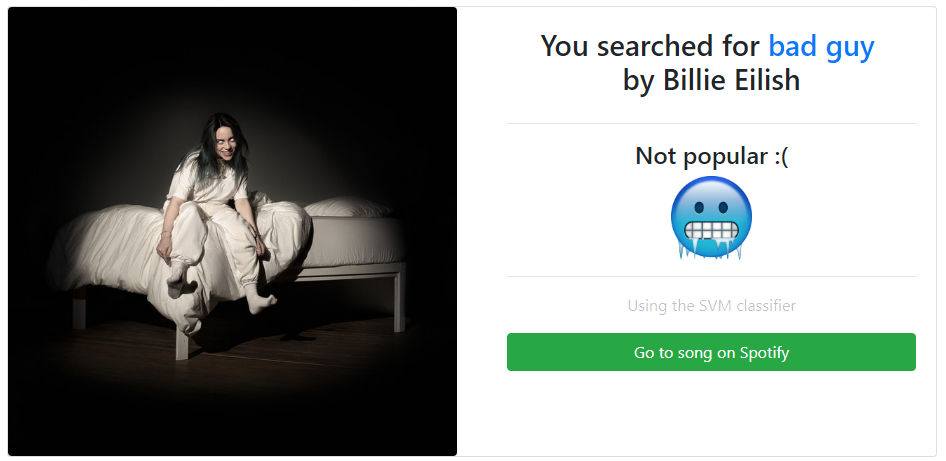
\includegraphics[width=0.7\textwidth]{web_application/fig/ui5.PNG} % second figure itself
\caption{The search performed page for the song "bad guy" by Billie Eilish}
\label{fig:ui4}
\end{figure}
%\chapter{Background}
In this chapter, a more thorough introduction to the research topic of this project is presented while also discussing related work in the area and introducing the Machine Learning concepts and techniques used.
\section{Hit Song Science}
Perhaps unsurprisingly, this research topic is quite a popular subject that has also gained some attention from the media. This is probably because a few companies have released products that they claimed were able to predict hit songs with high accuracy. This, as you can imagine, would be an invaluable tool for music producers and artists alike since they would be able to use it to their advantage and ultimately make a profit. However, it is unclear if those hit prediction tools actually worked and the implementation details were mostly kept secret.

This field of investigation has been referred to as Hit Song Science, a term coined by Mike McCready, founder of a music analysis company, and it aims to predict the success of songs before they are released on the market. However, as it turns out, there might be more to predicting the popularity of songs than just the features of the audio itself. Psychological aspects also come into play and a wide range of factors such as exposure, music marketing, media broadcasts, social influence play a role in whether we like a song or not. That is because what we listen to might be influenced by what our friends listen to, by what is played on radio/television or by what is being more heavily marketed. It is also usually the case that songs of popular artists will also be popular since they already have the exposure, while a new, unknown artist might struggle to get their songs on the radio since the popular songs get all the airtime (the rich get richer and poor get poorer). 

This makes the whole prediction problem even more complex than it was already. However, in Hit Song Science and, consequently, in this project, the goal is to look at the relation between features of the audio and the popularity of that song while disregarding these aforementioned complex and confusing psychological aspects. This problem then becomes similar to the prediction of stocks or the weather. Another way to look at this, as Pachet, puts it is "...as an idealistic attempt to determine the 'objective causes' of individual music preference, independently of the effects of social influence"  \cite{li_music_2011}.

\section{Related work}
\label{sec:relatedwork}
Research in this area has gone back and forth over time with some studies claiming that this kind of prediction might be possible and others saying that it is not. One of the earliest attempts is the work of Dhanaraj and Logan \cite{dhanaraj2005automatic}. They used general acoustic features (based on Mel-frequency cepstral coefficients) and features extracted from lyrics. To classify hits they used Support Vector Machines (SVMs) and boosting classifiers and for the data they used a database of 1700 songs. After the study, they concluded that there might indeed be something that distinguishes hits from non-hits and that audio based features and lyrically based features perform well on their own, but result in poorer performance when combined. 

Later, a larger scale and more complete study by Pachet and Roy \cite{pachet2008hit} contradicted their results. They used a database of 32000 songs with features from the MPEG-7 audio standard, a specific acoustic set generated with proprietary algorithms and a set of high-level metadata manually produced by humans. The classifier used was also SVM with an RBF kernel so the main differences were the features used and the size of the dataset. This study concluded that the popularity of songs cannot be learned from features of music titles, in this way contradicting the claims of Hit Song Science. This experiment could have put end to the debate on the topic due to its scale and level of completeness but as it turns out it might have had the opposite effect, fuelling even more experiments since it did not disprove the hypothesis completely \cite{li_music_2011}.

\begin{figure}[h]
\centering
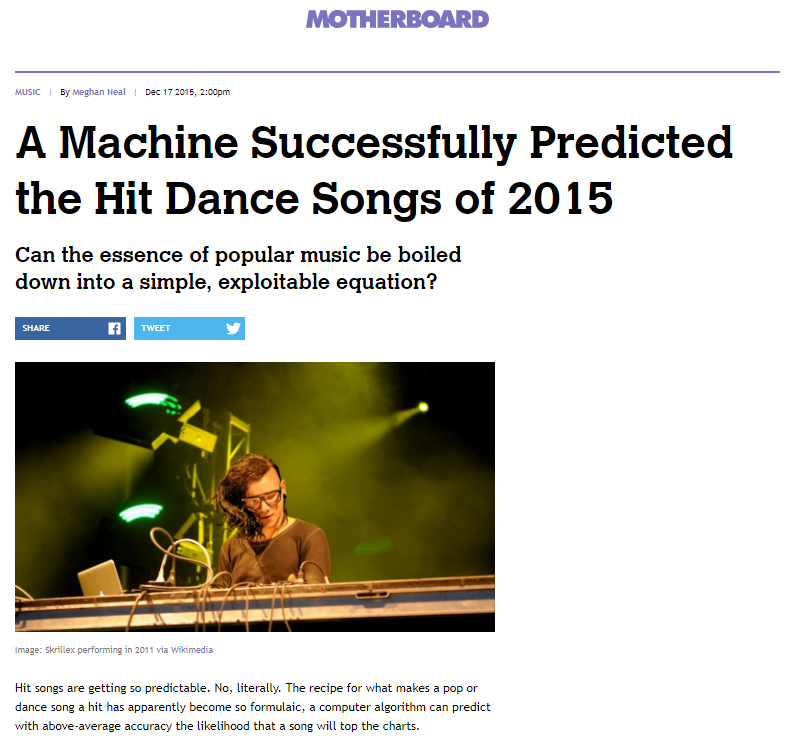
\includegraphics[width=0.50\linewidth]{background/fig/art2.PNG}
\caption{Online artice about the study of Herremans et al. \cite{herremans2014dance} \cite{MachineArticle:online}}
\label{fig:hitarticle}
\end{figure}

Trying to distinguish the top 5 from top 30-40 hits, Ni et al. \cite{ni2011hit} showed an experiment with more optimistic results due to the slightly different approach, the more novel audio features used (extracted from the EchoNest API, a music intelligence platform) and the classifier (a time-shifting perceptron). They claimed that hit song science might be a science once again. The research, however, does not include a lot of the perhaps important details of the implementation. Another study was conducted by Herremans et al. \cite{herremans2014dance} that looked at a similar approach, trying to predict if a song is a top 10 dance hit. Therefore, it only focused on a particular genre. The features were also obtained from The Echo Nest. They used models such as C4.5 trees, RIPPER rule set, logistic regression and SVMs, the best performing being the logistic regression model. This experiment again showed promising results concluding that predicting the popularity of dance songs is possible and is due to only using recent songs (so there is no need to account for the change in music taste over time), focusing on one genre and the features used.

More recently, Pham et al. \cite{pham2016predicting} used a subset of 2700 tracks from The Million Song Dataset \cite{bertin2011million} with features from this data set plus some from The Echo Nest. They compared different classifiers concluding that the SVM with an RBF kernel was the best performing one. Their aim was to also find the features that were more prominent in the prediction. Again, their study showed good results and the features that were more powerful predictors seem to have been the metadata ones rather than the acoustic ones since they seemed to reflect the trait of a song more accurately. An even more recent research by Reiman and Ornell \cite{reiman2018predicting} took an approach similar to the one in this project. They looked at predicting hit songs using four different classifiers with a data set of 600 tracks from the Billboard Hot 100 charts and features from the Spotify API. Their results were not as good as some of the previously presented experiments but were still slightly better than a random predictor.

\begin{figure}[h]
\centering
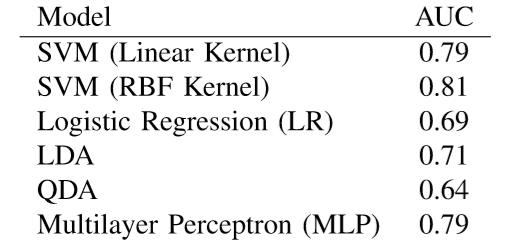
\includegraphics[width=0.7\linewidth]{background/fig/pic1.PNG}
\caption{Classifier AUC score results from the study of Pham et al. \cite{pham2016predicting}}
\label{fig:pham1}
\end{figure}

The results of these experiments seem promising overall making pursuing a different approach at this task worthwhile. While each research seems to have taken a slightly distinct path there were still certain common points. A few papers looked at models such as SVMs, logistic regression, naive bayes, multilayer perceptron, k-nearest neighbors and used features from The Echo Nest. This was a good starting point for my own study.

\section{Classification algorithms}
It seems clear now that some sort of prediction needs to be performed. To do that, this project uses machine learning which is used for the finding of patterns in data in an automated manner \cite{shalev2014understanding}. Nowadays,  we probably encounter machine learning every day when we search the internet, when shop online, even our phones might use it for unlocking using face recognition. It is truly all around us. 

But how do machines learn? Well, in a way similar to how animals or humans do, by using past experience to determine what to do in a new situation. In a very simple example of machine learning, that of filtering spam emails, the machine learning algorithm will be provided with a lot of examples of spam and non-spam messages. It will find patterns in these messages, such as the frequent occurrence of bad words in spam perhaps and when a new email arrives it will be able to tell if it is spam or not by using its 'past experience'. There are two main types of ways in which a machine can learn: supervised and unsupervised. 

Supervised learning applies in situations like the ones described above with the spam filter. Given a sample of messages that are labelled as spam and some labelled as not spam, when a new message arrives it can be labelled according to its similarity to a spam/non-spam message. In Figure \ref{fig:supunsup} a line (usually called a decision boundary) is drawn to separate the two classes. When a new point is plotted, it will be labelled according to which side of the decision boundary it is on.

On the other hand, in an unsupervised task the messages used for training are not labelled and so the algorithm needs to find patterns that separate the messages in a way, by clustering the data set into smaller subsets of similar messages, for example, like in Figure \ref{fig:supunsup} \cite{shalev2014understanding}. 

\begin{figure}[h]
\centering
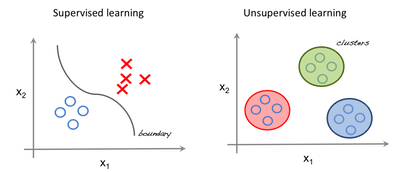
\includegraphics[width=0.9\linewidth]{background/fig/graph.png}
\caption{Supervised and unsupervised learning visualised \cite{SupervisedUnsupervised:online}}
\label{fig:supunsup}
\end{figure}

For the task in this project supervised learning will be used since we will provide the machine learning models with examples of songs that are labelled as popular or not popular. The model should then learn a certain pattern that differentiates popular songs from the less popular ones that it will then be able to apply to a previously unseen song and label it accordingly. 

As a starting point for choosing which classification algorithms to use, the related literature was reviewed. A few research papers used Support Vector Machines, Logistic Regression, Gaussian Naive Bayes, Multi-layer Perceptron and even K-Nearest Neighbours. Those were implemented to be able to compare results with previous work but other models were also tested such as Random Forests and AdaBoost. Below a succinct description of these models is provided.

Logistic regression is a machine learning technique that came from the field of statistics. It is at its core a mathematical modelling approach used to describe the relationship between a set of independent variables and a dependent variable. It is a very popular model because its output is a value between 0 and 1, value which describes a probability since it uses a sigmoid function (Equation \ref{eq:logreg}) to map predicted values to probabilities. The output represents the likelihood of the example belonging to class 1. For example, if predicting whether an individual has a disease or not, the probability will indicate how likely it is that the individual has that disease \cite{kleinbaum2002logistic}.

\begin{equation}
f(z)=\frac{1}{1+e^{-z}}
\label{eq:logreg}
\end{equation}

\addvbuffer[12pt 8pt]{
\begin{tabular}{lll}
	where & $e$ & is Euler's number,\\
	& $z$ & is the input to the function(the algorithm's prediction).\\

\end{tabular}
}


K-Nearest Neighbours is one of the simplest algorithms in machine learning, yet it is quite effective. To predict the class of a new given point, it looks at its k nearest neighbours (where k can range from 1 to the total number of points minus one and is usually chosen depending on the data). It then uses a majority vote to decide on the class of the new point \cite{16Neares99:online}.

Support Vector Machines are a "machine learning tool used for learning linear predictors in high dimensional feature spaces" \cite{shalev2014understanding}. It tries to find an optimal hyperplane to separate the given classes. The hyperplane is optimal when the distance between the hyperplane and the training examples is maximum. For example, in two dimensions the hyperplane would be a line that separates the points as seen in \autoref{fig:svm} and in three dimensions it would be a plane \cite{Introduc22:online}.

\begin{figure}[h]
\centering
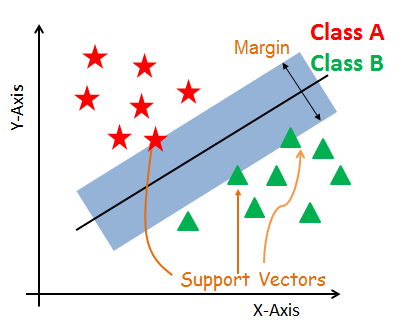
\includegraphics[width=0.6\linewidth]{background/fig/svm.PNG}
\caption{SVM application on 2D data \cite{SVMGraph:online}}
\label{fig:svm}
\end{figure}

The multi-layer perceptron (MLP) is a type of artificial neural network. As the name suggests, it is built upon the simpler perceptron which is a linear classifier that models a biological neuron. A multi-layer perceptron is composed of more than one perceptron which makes it able to solve more than just linear prediction tasks. An input layer receives the signal (the input data) and an output layer makes a decision based on the input. Between those two layers there can be any number of hidden layers that handle the bulk of the computation \cite{ABeginne87:online}.

The Naive Bayes classifiers are a family of simple probabilistic classifiers. Despite their simplicity they are very popular and have proven very effective. They use Bayes' theorem but with the added naive assumption that all the features are independent of each other, in other words, they assume conditional independence. This is considered a "naive" approach because it very rarely applies to the real world \cite{zhang2004optimality}. Gaussian Naive Bayes comes as an extension of the naive Bayes that adds the capability of handling continuous variables by making the assumption that the features are generated using a single Gaussian distribution \cite{john1995estimating} \cite{reiman2018predicting}.

The Random Forest or Random Decision Forest is an ensemble learning method, which means it uses multiple classifiers, in this case decision trees, to classify the data and then takes a majority vote of all those classifiers to decide on the class of an example. In this way, it mitigates the tendency of decision trees to overfit the data, improving the generalisation accuracy \cite{ho1995random}.

The AdaBoost classifer \cite{freund1997decision}, short for Adaptive Boosting, is a machine learning ensemble meta-algorithm that essentially tries to obtain a strong classifier from a set of weak ones. It trains a classifier on the data set and then creates new instances of that classifier that are trained on the same data set but the weights of incorrectly classified instances are adjusted (hence the adaptive title) \cite{sklearnadaboost:online}.

These algorithms were then implemented using the \textit{sci-kit learn} library \cite{pedregosa2011scikit} in Python. It is a module for machine learning that features various classification, regression and clustering algorithms including the ones mentioned above but also many more. Furthermore, it is designed to work with other numerical libraries in Python such as NumPy and SciPy. The code is run using Jupyter Notebooks \cite{kluyver2016jupyter}, a document format in which code from different languages can be executed. It is based around the IPython kernel which can run the Python code in Jupyter. It works in a browser and it provides a way of integrating code, explanations (in the form of text) and results (in the form of plots or graphics) in a single document which makes for easy reading, executing and understanding.

\section{Feature selection}

Feature selection is the process of removing the features that are not helpful to the predictor from the data. Often times this can improve the performance of the model since features that are not relevant can have a negative impact on the predictions. We are interested in only keeping the features that have the highest contribution to the desired output \cite{FeatureSel:online} \cite{guyon2003introduction}. There are three main types of methods used for feature selection: wrapper methods (use the model to score different feature subsets), filter methods (select feature subsets in the preprocessing phase, without using the model) and embedded methods (specific models can perform feature selection as part of training). 

Since the data only has 13 features the best feature subset can be found searching exhaustively by calculating a score for every possible feature combination and picking the best one. This is a wrapper method. There are therefore \(2^{13} - 1\) possible feature subsets and for each of them an AUC score is calculated using cross validation. Then the process is repeated for every model since the features chosen depend on the model used. The algorithm then looks like Algorithm \ref{alg3}.

\begin{figure}[h]
\centering
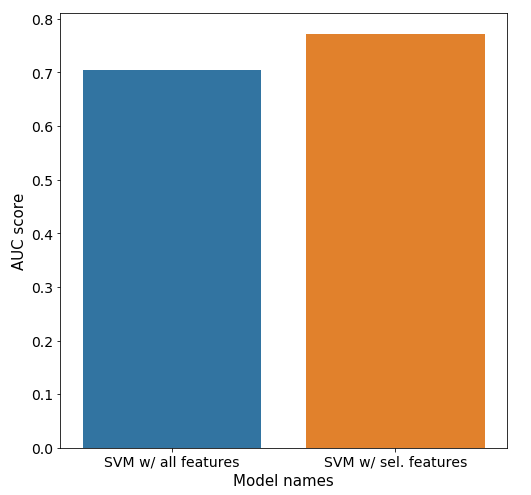
\includegraphics[width=0.8\linewidth]{background/fig/fs1.PNG}
\caption{AUC score for SVM before and after feature selection}
\label{fig:fs1}
\end{figure}

As an example, the performance increase for SVM can be seen in Figure \ref{fig:fs1} with the score plotted for the classification being performed on data with all the 13 features and on data with 7 selected features (energy, tempo, speechiness, instrumentalness, time signature, duration, loudness). It is about a 7\% increase which may not be much but the reduction of features leads to a much simpler model, the number of features being almost halved.

\begin{algorithm}[caption={"Feature selection algorithm"}, label={alg3}]
begin
    foreach model in the model list
      foreach possible feature subset
        do cross validation
          calculate AUC score for each iteration
        end
        calculate average AUC score for all iterations
        store feature set and score in a list
      end
      pick subset with best score for model
    end
end
    
\end{algorithm}

\section{Imbalanced classes}
\label{sec:imbalance}
Early on when trying to evaluate the models the results seemed unusually high. That was because I was only looking at the prediction accuracy of the models which is the percentage of correct predictions. That was a problem since almost 90\% of the data set is of class 0 and only 10\% of class 1 so it is highly imbalanced (this can be observed in Figure \ref{fig:imbalance}). This meant that if the model predicted everything as class 0 it would have a 90\% accuracy even though it failed to identify any of the hits which is what we are actually interested in. To mitigate this problem a few different approaches were tried: using over-sampling, adjusting class weights in models and looking at different scoring metrics (discussed in Section \ref{sec:evalation}).

\begin{figure}[h]
\centering
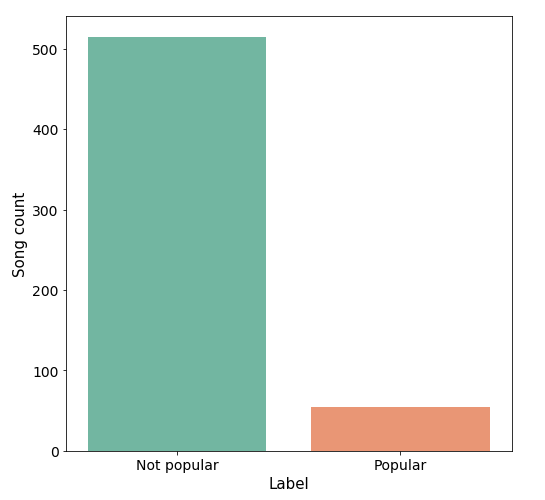
\includegraphics[width=0.7\linewidth]{background/fig/imbalance.PNG}
\caption{Plot of number of examples for each class in the data set}
\label{fig:imbalance}
\end{figure}

Over-sampling is a technique used to create more examples of the minority class to make the data set balanced. A common way to do so was to just duplicate the examples of the minority class, but this can easily lead to overfitting. A better approach is SMOTE (Synthetic Minority Over-sampling Technique) \cite{chawla2002smote}, a technique used to create new "synthetic" samples by using an algorithm similar to k-nearest neighbours that creates a new example and randomly sets its feature values based on those of the neighbours. 

Another technique that can be used to mitigate this problem involves adjusting the model to penalise a misclassification of a sample of class 1 more than one for class 0. This can be done by adjusting the weights of the classes and some models in sci-kit learn support a parameter that sets the weights automatically according to the balance of samples in the data set.

Both of these options were used and compared to ensure the best solution was chosen. The scores were similar with slightly higher results when adjusting the weights but since that was not available for every model, over-sampling also had to be used. 


\chapter{Conclusion}

In this chapter, the outcomes of this experiment are presented and further improvements to this work along with some learning outcomes from this experience are discussed.

\section{Summary of achievements}
\begin{itemize}
\item Achieved good prediction scores that conclude it is possible to predict hit songs just based on the features of the audio.
\item With a score of 0.77 after optimisation and feature selection, SVMs are able to predict popular songs with a good degree of accuracy and do quite a bit better than a random predictor.
\item With the feature selection process I was able to find some of the features that had a greater impact on the prediction and even though they depend on the model some of the more common ones are energy, loudness, tempo and duration.
\item The web application implemented also allows users to see the predictions of this model and a few others on any song on Spotify in real time and could be used as a tool for artists or music labels.
\end{itemize}

% The results achieved in this experiment are promising and hint towards the possibility of there actually being a common pattern among hit songs. With an score of 0.77, SVM are able to predict popular songs with a good degree of accuracy and do quite a bit better than a random predictor. Therefore we can conclude that predicting popular music might indeed be possible just based on features of the audio. With the feature selection process I was able to find some of the features that had a greater impact on the prediction. Although they depend on the model, some of the more common ones were energy, loudness, tempo and duration. The web application implemented also allows users to see the predictions of this model and a few others on any song on Spotify in real time.

\section{Further improvements}

The data set used is rather small and it is not really representative of the very wide variety of genres and sounds present in the world of music. Also, the data sample contains songs that are fairly recent so the results in this study might not apply in the future, unless the models will be trained again on different data sampled at that time. 

I believe that further research in this area should try to use a larger data set. I have started along this path later on in the research, getting a bigger data set of 3000 songs by scraping a charts website \cite{SpotifyCharts:online} and also getting the same features for those songs. Using the same models on this data showed poorer results than on the smaller set which might be due to the new examples making it harder for the models to find patterns rather than helping it.

Another possible improvement that could be made is looking at different definitions of popularity. In Section \ref{ground_truth} I mentioned that the Spotify popularity metric was used for that in this research. Later on, I looked into using the view count on Youtube and wrote a Python script to match the songs in the data set from Spotify with their corresponding Youtube video and get the views for it using the Youtube API (the correlation between popularity and view count can be seen in Figure \ref{fig:ytcor}). For the larger data set, the charts website \cite{SpotifyCharts:online} also provided a number of total streams (essentially the total number of plays a song had on Spotify) which was also added. Using different combinations of popularity and Youtube view count or the view count, popularity and total stream numbers did not seem to improve the results. However, there are still a few other ways of defining a popular song not explored in this research but were used in previous work such as appearance on Billboard Top 100 or charts from the Official Charts Company. Another idea would be to use the number of Shazams \cite{wang2006shazam} (Shazam is a music recognition software that is widely used to identify songs) since that might provide an indication of what songs people like so much that they want to find out the name of the song immediately. 

Furthermore, the number of features used in this project is quite small as compared to other research so I think this is a clear path for improvement. Some signal processing could be done to extract other useful features from the raw audio or something like sentiment analysis could be performed on social networks such as Twitter or Facebook to see if the song gets any attention but the latter would need to happen after the song's release.

\section{What I would do differently?}

If I were to start this project again I would probably spend more time on the planning of the project. Although I had a plan at the beginning, when I started researching the project and learned more about the task, more research paths came up that took time to explore. Therefore, I did not respect the plan at times, mixing research with implementation, for example, but I learned how to adjust over time. With a more carefully thought out plan, I think I could have been more efficient and could have explored more additional functionalities but now I have at least acquired the experience to do so for further projects. 

I would also ask my supervisor more about the technologies encountered in the project, since I feel like I didn't take full advantage of his expertise on the subject and I could have learned even more from him.

Another aspect that I would approach differently is I would also start out with a bigger data set. Because I did not have experience with working with data and machine learning I did not know where or how to get a bigger data set and so I created my own one. This was good for a small scale experiment but later I found out sources with larger, already compiled data sets.



\appendix
\chapter{First Appendix}
\section{Feature description}
The information in this table is from the Spotify Web API website \cite{SpotifyFeatures:online}.

\begin{longtable}{|p{3cm}|p{1.6cm}|p{7cm}|}
% \begin{tabular}{|p{3cm}|p{2cm}|p{7cm}|}
\hline
\textbf{Feature name}     & \textbf{Feature type} & \textbf{Feature description}                                                                                                                                                                                                                                                                                                                                                                                                                                                                                                \\ \hline \hline
\endhead
duration\_ms     & int          & The duration of the track in milliseconds.                                                                                                                                                                                                                                                                                                                                                                                                                                                                         \\ \hline
key              & int          & The estimated overall key of the track. Integers map to pitches using standard Pitch Class notation . E.g. 0 = C, 1 = C♯/D♭, 2 = D, and so on. If no key was detected, the value is -1.                                                                                                                                                                                                                                                                                                                            \\ \hline
mode             & int          & Mode indicates the modality (major or minor) of a track, the type of scale from which its melodic content is derived. Major is represented by 1 and minor is 0.                                                                                                                                                                                                                                                                                                                                                    \\ \hline
time\_signature  & int          & An estimated overall time signature of a track. The time signature (meter) is a notational convention to specify how many beats are in each bar (or measure).                                                                                                                                                                                                                                                                                                                                                      \\ \hline
acousticness     & float        & A confidence measure from 0.0 to 1.0 of whether the track is acoustic. 1.0 represents high confidence the track is acoustic.                                                                                                                                                                                                                                                                                                                                                                                       \\ \hline
danceability     & float        & Danceability describes how suitable a track is for dancing based on a combination of musical elements including tempo, rhythm stability, beat strength, and overall regularity. A value of 0.0 is least danceable and 1.0 is most danceable.                                                                                                                                                                                                                                                                       \\ \hline
energy           & float        & Energy is a measure from 0.0 to 1.0 and represents a perceptual measure of intensity and activity. Typically, energetic tracks feel fast, loud, and noisy. For example, death metal has high energy, while a Bach prelude scores low on the scale. Perceptual features contributing to this attribute include dynamic range, perceived loudness, timbre, onset rate, and general entropy.                                                                                                                          \\ \hline
instrumentalness & float        & Predicts whether a track contains no vocals. “Ooh” and “aah” sounds are treated as instrumental in this context. Rap or spoken word tracks are clearly “vocal”. The closer the instrumentalness value is to 1.0, the greater likelihood the track contains no vocal content. Values above 0.5 are intended to represent instrumental tracks, but confidence is higher as the value approaches 1.0.                                                                                                                 \\ \hline
liveness         & float        & Detects the presence of an audience in the recording. Higher liveness values represent an increased probability that the track was performed live. A value above 0.8 provides strong likelihood that the track is live.                                                                                                                                                                                                                                                                                            \\ \hline
loudness         & float        & The overall loudness of a track in decibels (dB). Loudness values are averaged across the entire track and are useful for comparing relative loudness of tracks. Loudness is the quality of a sound that is the primary psychological correlate of physical strength (amplitude). Values typical range between -60 and 0 db.                                                                                                                                                                                       \\ \hline
speechiness      & float        & Speechiness detects the presence of spoken words in a track. The more exclusively speech-like the recording (e.g. talk show, audio book, poetry), the closer to 1.0 the attribute value. Values above 0.66 describe tracks that are probably made entirely of spoken words. Values between 0.33 and 0.66 describe tracks that may contain both music and speech, either in sections or layered, including such cases as rap music. Values below 0.33 most likely represent music and other non-speech-like tracks. \\ \hline
valence          & float        & A measure from 0.0 to 1.0 describing the musical positiveness conveyed by a track. Tracks with high valence sound more positive (e.g. happy, cheerful, euphoric), while tracks with low valence sound more negative (e.g. sad, depressed, angry).                                                                                                                                                                                                                                                                  \\ \hline
tempo            & float        & The overall estimated tempo of a track in beats per minute (BPM). In musical terminology, tempo is the speed or pace of a given piece and derives directly from the average beat duration. \\ \hline
% \end{tabular}
\caption{Table containing feature description}
\label{tab:feature}
\end{longtable}

% Fix to move content to next page
\vspace{300pt}

\section{Additional figues}
\begin{figure}[h]
\centering
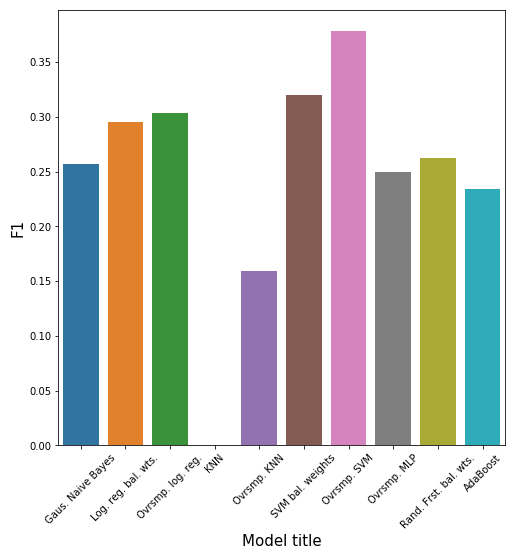
\includegraphics[width=0.62\linewidth]{appendix/fig/f1s.PNG}
\caption{Model F1 scores}
\label{fig:f1s}
\end{figure}
% \vspace{-700pt}
\begin{figure}[h]
\centering
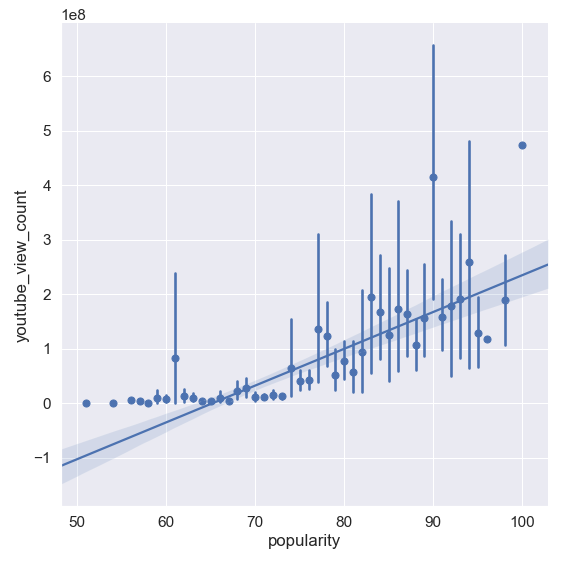
\includegraphics[width=0.62\linewidth]{appendix/fig/correlation.PNG}
\caption{Youtube view count and popularity correlation}
\label{fig:ytcor}
\end{figure}

% \section{Full scores table}

% This is a table presenting all the different evaluation metrics used for every model. It looks at Accuracy, Specificity, Recall, Precision, F1 score, AUC and Generalisation AUC.

% On top of Accuracy, Specificity, Recall, Precision, F1 score and AUC this table also includes Average Precision (AP). It is meant to summarise the precision-recall curve (a curve similar to the ROC curve but it plots Precision and Recall for every threshold instead of Recall and False Positive Rate). It is supposed to be a good indication of model performance in imbalanced data sets. A more in-depth description is found in the sci-kit learn documentation \cite{sklearnAP:online}.

% \begin{table}
% % \begin{adjustbox}{max width=\textwidth}
% \resizebox{\textwidth}{!}{%
% \begin{tabular}{*{8}{|c}|}
% \hline
% \textbf{Model title}    & \textbf{Acc.} & \textbf{Spec.} & \textbf{Rec.} & \textbf{Prec.} & \textbf{F1} & \textbf{AUC} & \textbf{Gen. AUC}\\ \hline
% Gaussian Naive Bayes    & 0.404             & 0.339                & 0.940                        & 0.149              & 0.257       & 0.670        & 0.421                           \\ \hline
% Log. reg. bal. weights. & 0.639             & 0.634                & 0.680                        & 0.191              & 0.296       & 0.745        & 0.433                          \\ \hline
% Over-sampling log. reg.  & 0.641             & 0.632                & 0.720                        & 0.194              & 0.304       & 0.730        & 0.454                           \\ \hline
% KNN                     & 0.891             & 1.000                & 0.000                        & 0.000              & 0.000       & 0.560        & 0.685                           \\ \hline
% Over-sampling KNN        & 0.739             & 0.802                & 0.220                        & 0.130              & 0.159       & 0.511        & 0.478                           \\ \hline
% SVM bal. weights        & 0.628             & 0.607                & 0.800                        & 0.203              & 0.320       & {\ul 0.772}  & 0.566                          \\ \hline
% Over-sampling SVM        & 0.743             & 0.749                & 0.700                        & 0.270              & {\ul 0.378} & 0.770        & 0.481                          \\ \hline
% Over-sampling MLP        & 0.843             & 0.915                & 0.260                        & 0.248              & 0.250       & 0.693        & 0.572                          \\ \hline
% Random Forest bal. wts. & 0.733             & 0.768                & 0.440                        & 0.190              & 0.262       & 0.676        & 0.382                           \\ \hline
% AdaBoost                & 0.843             & 0.917                & 0.240                        & 0.235              & 0.234       & 0.633        & 0.486                           \\ \hline
% \end{tabular}%
% }
% \caption{Table containing model scores}
% \label{tab:modelscores}
% \end{table}

% \begin{longtable}{|p{2.5cm}|p{1cm}|p{1cm}|p{1cm}|p{1cm}|p{1cm}|p{1cm}|p{1cm}|p{1cm}|}
% \hline
% \textbf{Model title}    & \textbf{Acc.} & \textbf{Spec.} & \textbf{Rec.} & \textbf{Prec.} & \textbf{F1} & \textbf{AUC} & \textbf{Gen. AUC}\\ \hline
% Gaussian Naive Bayes    & 0.404             & 0.339                & 0.940                        & 0.149              & 0.257       & 0.670        & 0.421                           \\ \hline
% Log. reg. bal. weights. & 0.639             & 0.634                & 0.680                        & 0.191              & 0.296       & 0.745        & 0.433                          \\ \hline
% Over-sampling log. reg.  & 0.641             & 0.632                & 0.720                        & 0.194              & 0.304       & 0.730        & 0.454                           \\ \hline
% KNN                     & 0.891             & 1.000                & 0.000                        & 0.000              & 0.000       & 0.560        & 0.685                           \\ \hline
% Over-sampling KNN        & 0.739             & 0.802                & 0.220                        & 0.130              & 0.159       & 0.511        & 0.478                           \\ \hline
% SVM bal. weights        & 0.628             & 0.607                & 0.800                        & 0.203              & 0.320       & {\ul 0.772}  & 0.566                          \\ \hline
% Over-sampling SVM        & 0.743             & 0.749                & 0.700                        & 0.270              & {\ul 0.378} & 0.770        & 0.481                          \\ \hline
% Over-sampling MLP        & 0.843             & 0.915                & 0.260                        & 0.248              & 0.250       & 0.693        & 0.572                          \\ \hline
% Random Forest bal. wts. & 0.733             & 0.768                & 0.440                        & 0.190              & 0.262       & 0.676        & 0.382                           \\ \hline
% AdaBoost                & 0.843             & 0.917                & 0.240                        & 0.235              & 0.234       & 0.633        & 0.486                           \\ \hline
% \caption{Table containing model scores}
% \label{tab:modelscores}
% \end{longtable}


\bibliographystyle{unsrt}
\bibliography{bibs/sample}
\addcontentsline{toc}{chapter}{Bibliography}

\end{document}